\documentclass[11pt,a4paper]{article}
\usepackage[margin=2cm]{geometry}
\usepackage{graphicx}
\usepackage{booktabs}
\usepackage{amsmath}
\usepackage{amssymb}
\usepackage{siunitx}
\usepackage[hidelinks]{hyperref}
\usepackage{caption}
\usepackage{subcaption}
\usepackage{float}
\usepackage{enumitem}
\captionsetup{font=small}
\setlist[itemize]{nosep, leftmargin=1.2em}
\setlength{\parskip}{3pt}

\title{Conditional diffusion emulator of Veros ACC equilibrium states:\\results}
\author{}
\date{5 October 2026}

\begin{document}
\maketitle

\section*{Summary}
\begin{itemize}
  \item Goal: generate the post-spin-up $(T, S)$ state of the Veros ACC channel from the EKE-closure
        coefficients $(c_k, c_\epsilon)$, skipping the spin-up.
  \item Pipeline: DINO-Fusion diffusion code adapted to a parameter ensemble, with a velocity target, an
        unclipped sampler and the loss restricted to the water cells; one split runs end to end in under one
        A100 hour. A first round with DINO-Fusion's $\epsilon$-prediction and clipped sampler gave
        0.06--\SI{0.15}{K} on the same splits; the present configuration is better on every metric and is used
        throughout.
  \item Interpolation (scattered points, a band of three rows, the $5\times5$ and $7\times7$ centre blocks held
        out): hold-out RMSE 0.029 / 0.048 / 0.037 / \SI{0.041}{K} against 0.037 / 0.116 / 0.077 / \SI{0.114}{K}
        for the nearest training run and 0.155--\SI{0.197}{K} for the mean state. The model's error does not
        depend on the size of the gap; the baselines' does, so the model wins as soon as the gap exceeds one
        grid step.
  \item Extrapolation (the 51 or 75 outer runs held out, training on the centre; the top row): 0.079 / 0.123 /
        \SI{0.074}{K} against 0.131 / 0.155 / \SI{0.170}{K}, medians 0.041 / 0.049 / 0.054. The mean is set by the
        warm corner, where the model is cold-biased (corner run 0.61, 1.05 and \SI{0.21}{K} when it lies two,
        three and one cells from the training set); elsewhere 0.03--\SI{0.15}{K}.
  \item Four training runs only, one step in from each corner: 0.150 vs \SI{0.179}{K} for the nearest run and
        $W_1$ 0.090 vs \SI{0.156}{K}; the model interpolates the warm-side trend the baseline cannot, and loses
        where the state hardly changes.
  \item Samples: single-sample RMSE 0.07--\SI{0.11}{K} in interpolation, ensemble spread 0.05--\SI{0.07}{K} against
        a true within-window \SI{0.03}{K}; $S$ within \SI{0.05}{psu} of its constant; land exact.
  \item Physical miss: temperature inversions are generated at the rate of the weakly eddying runs in every
        regime.
\end{itemize}

\section{Data}
\begin{itemize}
  \item 100 Veros ACC runs on a $10\times10$ log-spaced grid, $c_k\in[0.0125,\,0.8]$,
        $c_\epsilon\in[0.0875,\,5.6]$; 100 years, 30-day output; interior grid $30\times42\times15$ (x, y, z).
  \item Kept: $T$ and $S$, last 20 years (241 snapshots per run). $S = \SI{35}{psu}$ everywhere in every run.
  \item Nearly deterministic end states: within-window std \SI{0.01}{K} above \SI{1400}{m} vs
        \SI{0.05}{K} between grid neighbours; the bottom level still drifts by \SI{0.45}{K} over the window.
  \item One effective parameter: $\log c_k - 1.05\,\log c_\epsilon$ explains 99\,\% of the variance of the
        domain-mean $T$; the low-$c_k/c_\epsilon$ part of the grid saturates.
  \item Per-level distribution of $T$ (Figure~\ref{fig:tdist}): above \SI{400}{m} a mixture of restoring
        values and interior, with $\sigma_z$ set by the meridional gradient, so $\mu_z \pm 3\sigma_z$ is wider than
        the level and the normalised values stay within $[-0.85,\,0.6]$; below \SI{1400}{m} a warm tail to
        $x' = +2.7$. Run-to-run signal $\sigma_z^{\mathrm{runs}}$: 0.7\,\% of $3\sigma_z$ at the surface, 26\,\% at
        the bottom. The narrow peaks are the zonally uniform southern rows $y = 0$--$6$, the restoring zone: one
        peak per row, at the same value in every run to within 0.04--\SI{0.18}{K} (Figure~\ref{fig:rows}).
\end{itemize}

\begin{figure}[!htb]
\centering
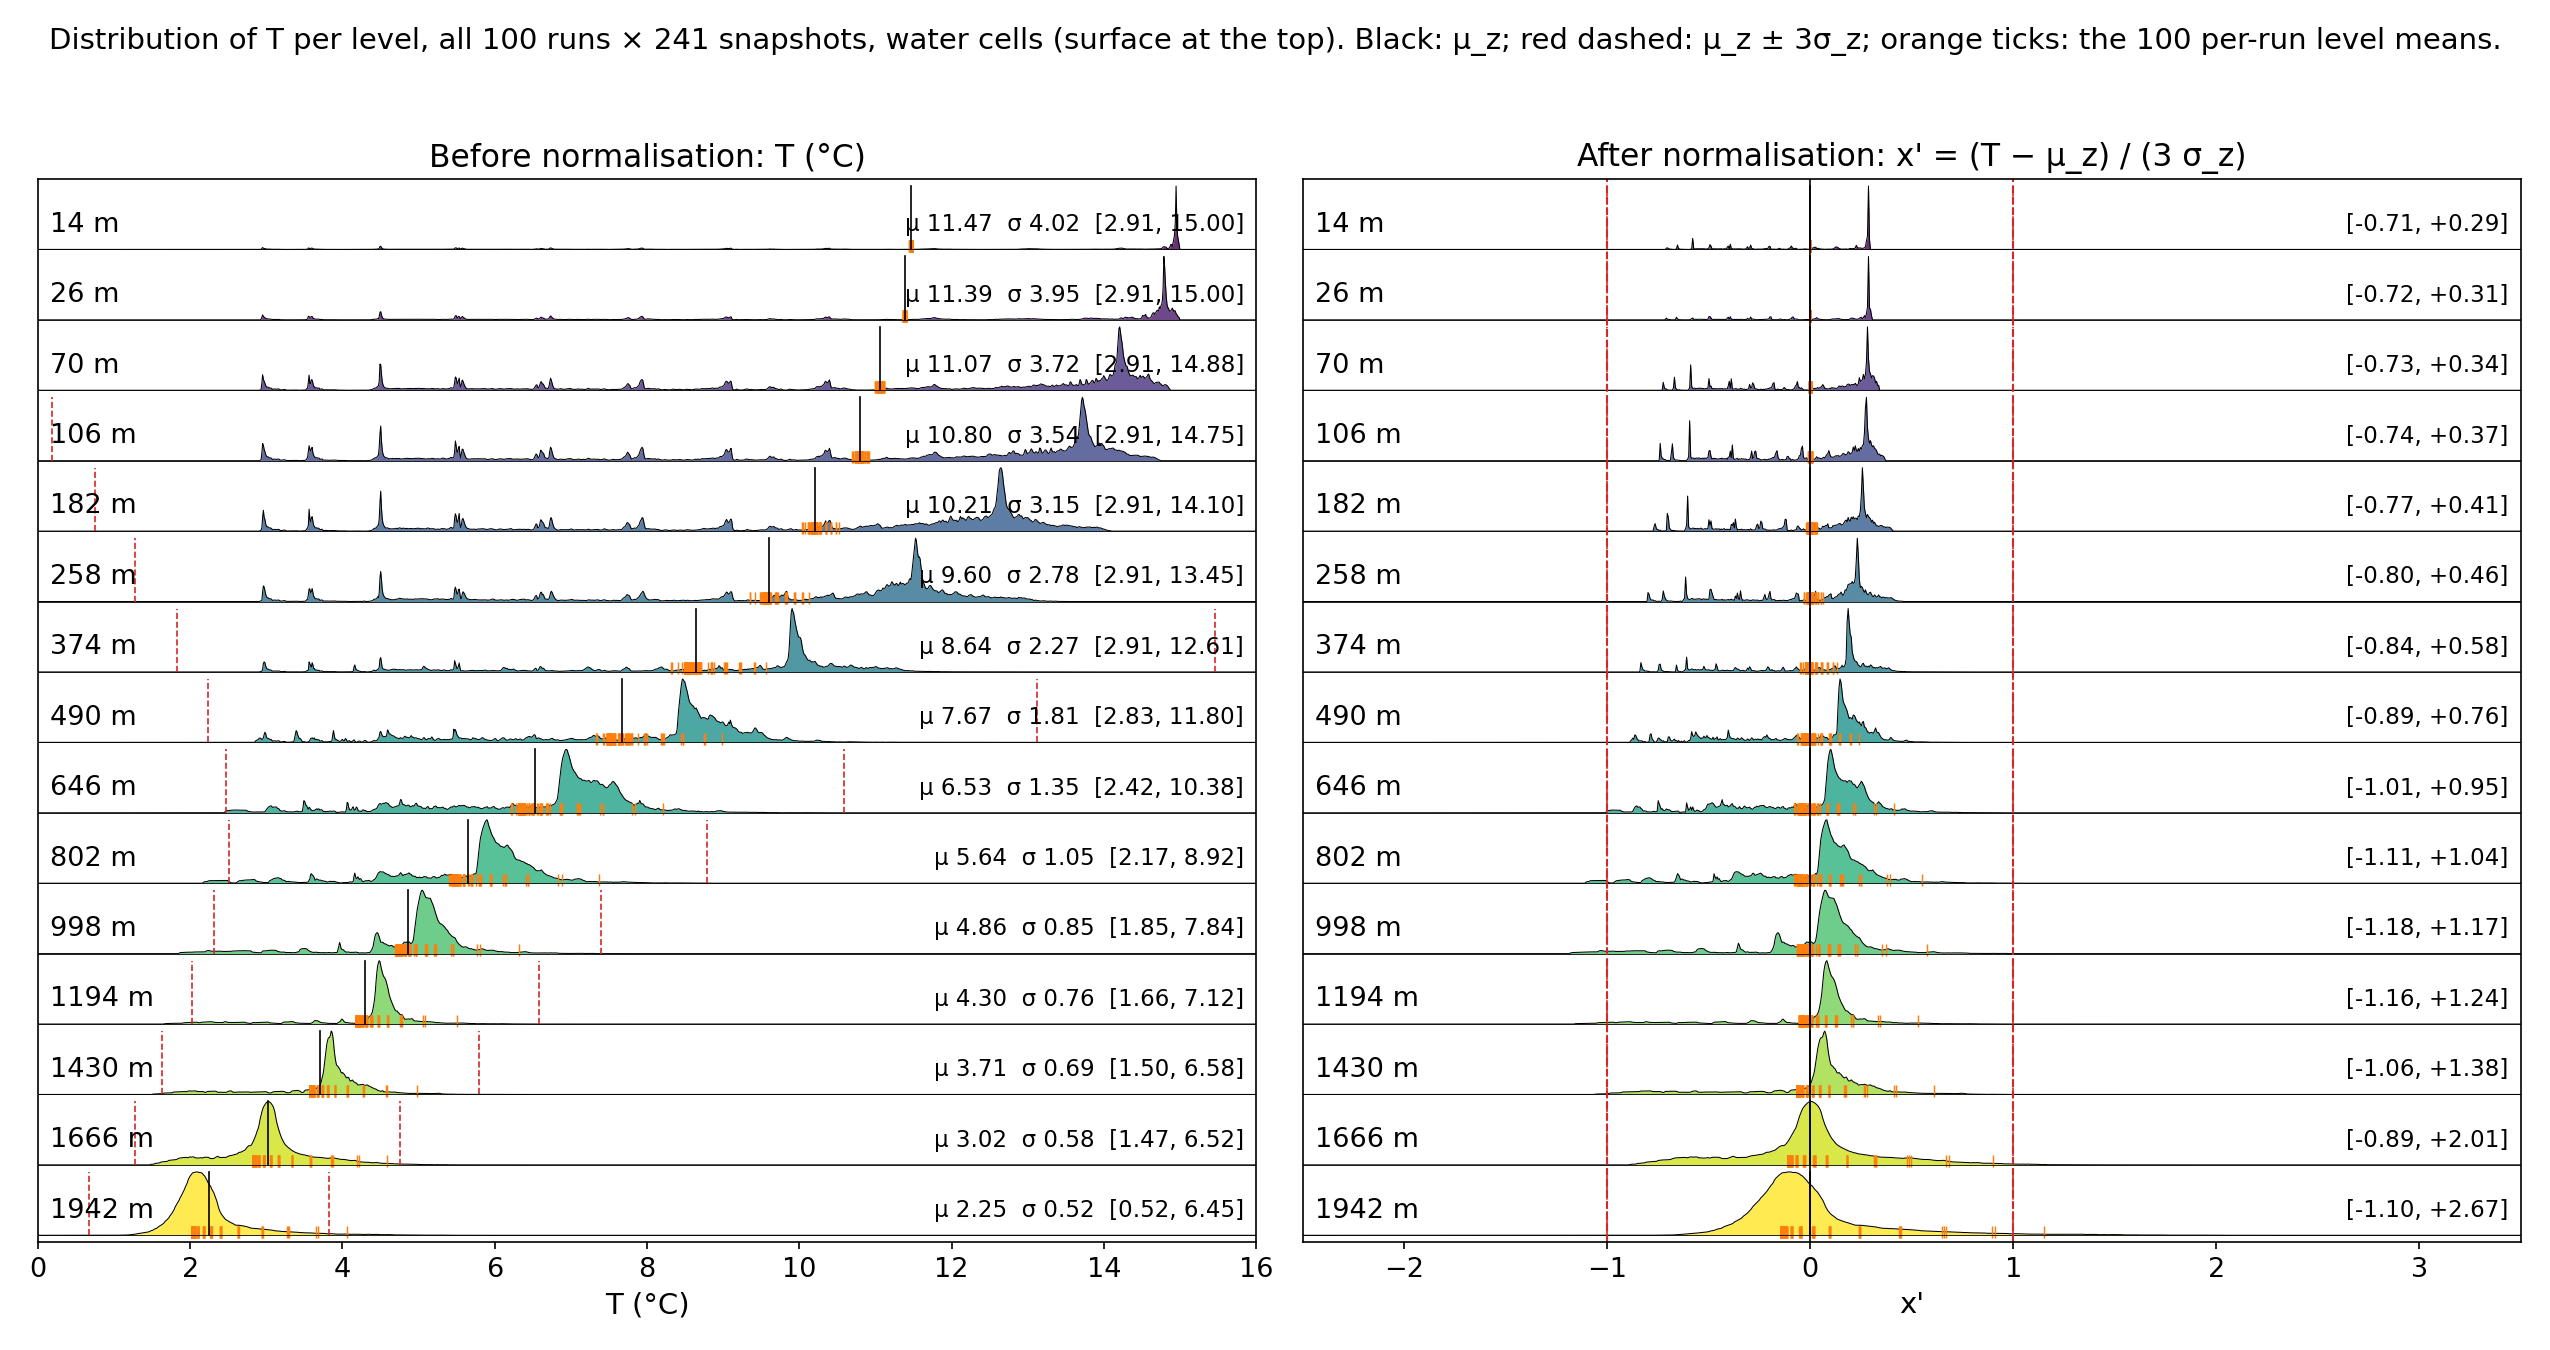
\includegraphics[width=\textwidth]{../data/T_distribution_per_level.png}
\caption{Distribution of $T$ per level over all 100 runs and 241 snapshots (water cells), before (left) and after
(right) the per-level normalisation of Eq.~(\ref{eq:norm}). Black: $\mu_z$; red dashed: $\mu_z \pm 3\sigma_z$;
orange ticks: the 100 per-run level means.}
\label{fig:tdist}
\end{figure}

\begin{figure}[!htb]
\centering
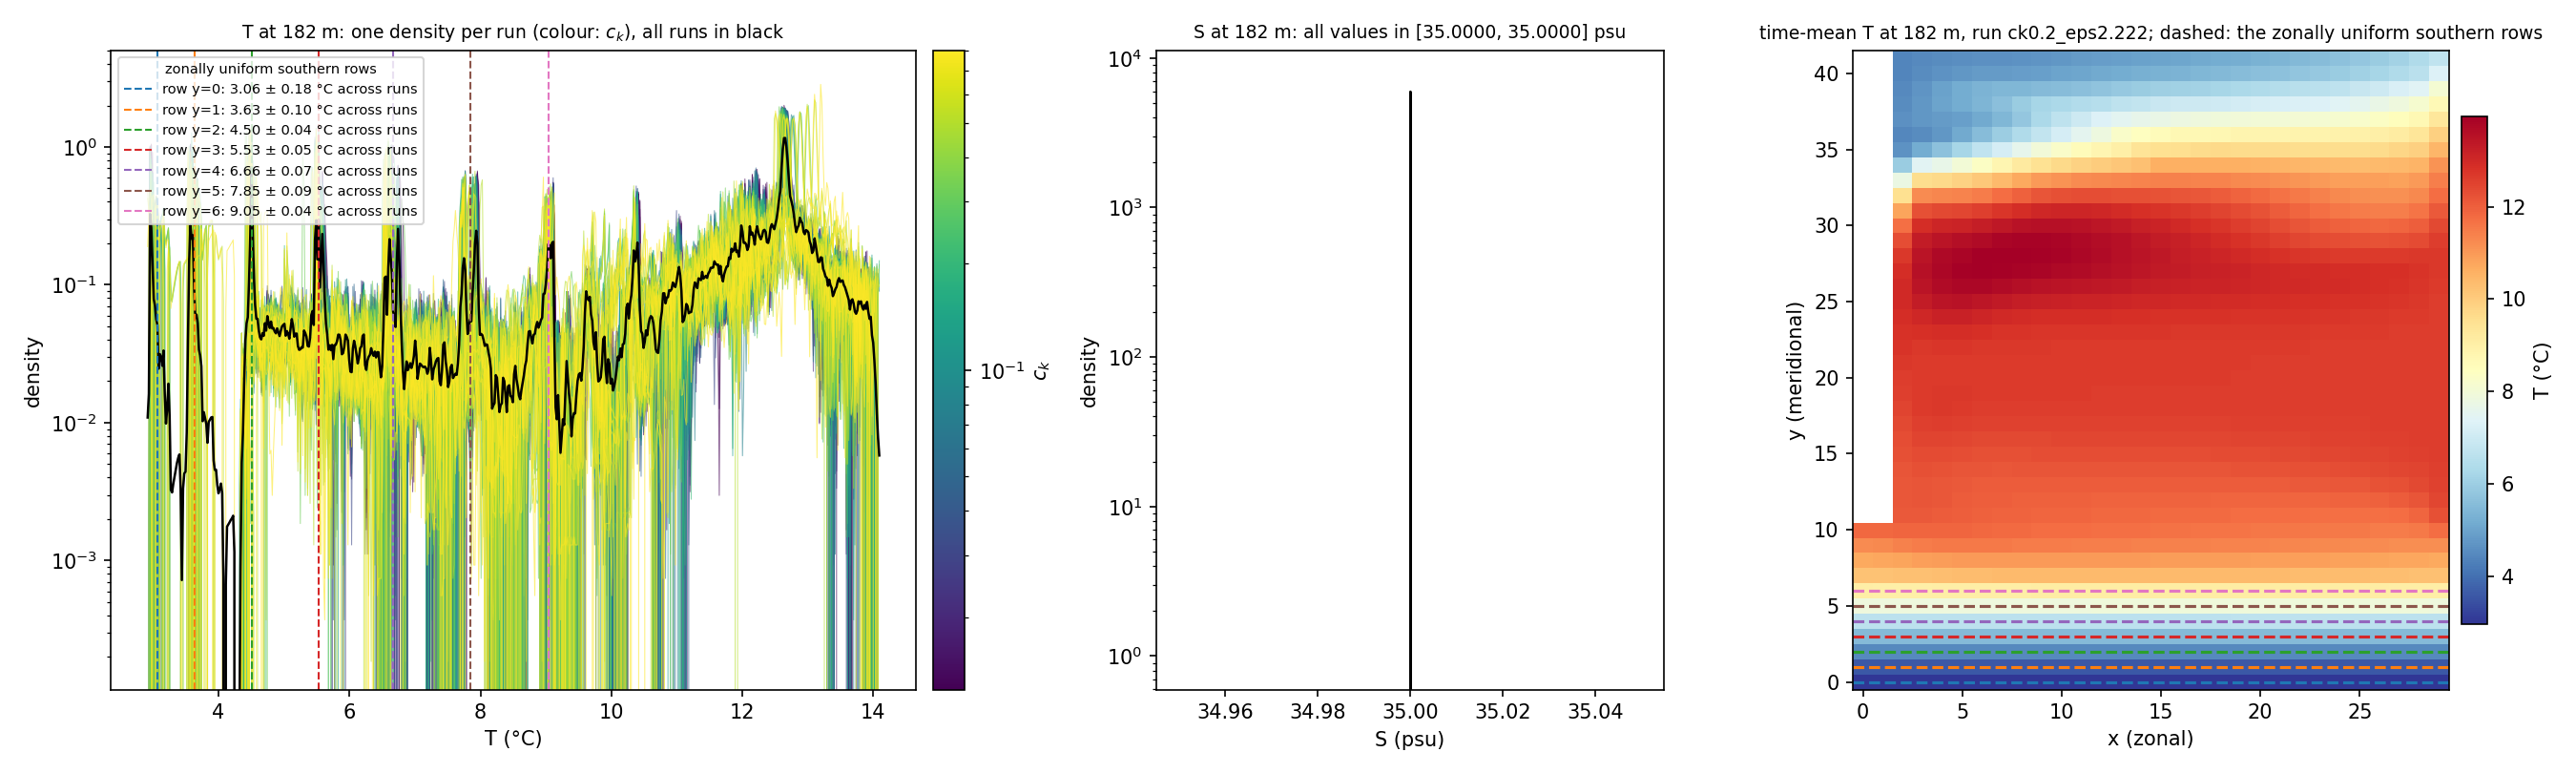
\includegraphics[width=\textwidth]{../data/level_density_150m.png}
\caption{The level nearest \SI{150}{m} (\SI{182}{m}), last 20 years, water cells. Left: one density of $T$ per run
(colour: $c_k$; log scale), all runs in black; dashed: the zonal-mean $T$ of the southern rows $y = 0$--$6$, each
with its spread across runs. Middle: $S$, exactly \SI{35}{psu} everywhere. Right: time-mean $T$ of one run at
that level with the same rows marked. Every narrow peak of the distribution is one southern row.}
\label{fig:rows}
\end{figure}

\section{Method}
\begin{itemize}
  \item Fields $\to$ 30 channels $(T_{1..15}, S_{1..15})$, normalised per level, land $\to 0$,
        zero-padded $42\times30 \to 48\times32$:
        \begin{equation}
          x'_{z} = \frac{x_{z} - \mu_{z}}{3\,\max(\sigma_{z}, 0.05)} .
          \label{eq:norm}
        \end{equation}
        $\mu_z, \sigma_z$ are computed once on all 100 runs and held fixed for every split (a deliberate, mild
        leakage of 30 scaling constants; no held-out state enters training).
  \item Denoiser: UNet2DModel (64, 64, 128, 128), 6.9\,M parameters. The condition $c$, the standardised pair
        $(\log c_k, \log c_\epsilon)$, enters through an MLP added to the timestep embedding.
  \item DDPM with the velocity target, 1000 steps, squared-cosine schedule, EMA; the loss runs over the water
        cells only:
        \begin{equation}
          \mathcal L(\theta) = \mathbb E_{t,\,x_0,\,\epsilon}\,
          \big\| v_t - v_\theta(x_t, t, c) \big\|^2_{\mathrm{water}}, \qquad
          x_t = \sqrt{\bar\alpha_t}\,x_0 + \sqrt{1-\bar\alpha_t}\,\epsilon, \quad
          v_t = \sqrt{\bar\alpha_t}\,\epsilon - \sqrt{1-\bar\alpha_t}\,x_0 .
        \end{equation}
        20\,000 steps, batch 32, AdamW $10^{-4}$ with cosine decay; 17--\SI{25}{min} on one A100.
  \item Sampling: 1000-step DDPM loop with EMA weights; the clean-state estimate
        $\hat x_0 = \sqrt{\bar\alpha_t}\,x_t - \sqrt{1-\bar\alpha_t}\,\hat v$ is used unclipped; after every step
        the land and padding cells are reset to zero at the step's noise level, $\sqrt{1-\bar\alpha_t}\,z$, as in
        training. 32 samples per condition.
  \item Why the velocity target and the water-only loss. With $\epsilon$-prediction the clean-state estimate
        divides by $\sqrt{\bar\alpha_t}$, so the chain needs a clip on $\hat x_0$, and the clip at $|x'| \le 1$
        caps the deep levels, whose data reach $+2.7$; the velocity form stays bounded and runs unclipped. Its
        target, however, has a step at the land and padding border (noise only there, noise minus the clean state
        in the water), and with the loss on all cells the network built that step with a localised activation
        spike in its decoder: a $3\times3$ patch of wrong values, 0.3--\SI{0.9}{K} through the water column, at a
        seed-dependent place next to a zero border, invisible to the loss. Restricting the loss to the water cells
        removes the step and the spike (Figure~\ref{fig:spot}); the evaluation summary flags any such patch
        (worst column of the single-sample error and the zonal correlation of its error).
\end{itemize}

\paragraph{Differences from the DINO-Fusion code.}
\begin{itemize}
  \item Conditioning: DINO's UNet is unconditional and is steered at sampling time by constraints; here the UNet
        receives $(\log c_k, \log c_\epsilon)$ through the timestep embedding, and the data are an ensemble of 100
        runs split by run instead of one trajectory.
  \item Sampling: DINO's BorderZeroConstraint resets land and padding to exact zeros after every step, which the
        network never sees in training, where those cells carry noise like every other. Here they are reset to
        zeros at the step's noise level, $\sqrt{1-\bar\alpha_t}\,z$, exactly as in training. DINO's stratification
        constraints are not ported yet.
  \item Training target: velocity instead of noise, loss on the water cells only, no clip at sampling.
  \item Everything else is kept: transform chain, 3-std normalisation, DDPM settings, EMA.
\end{itemize}

\section{Evaluation}
\begin{itemize}
  \item Truth: 20-year time-mean state of each held-out run; metrics on water cells.
  \item Baselines: mean training state; nearest training run in standardised log-parameter space; average of
        the axis-neighbour training runs on the grid.
  \item Eight hold-out splits, same data file and statistics, different training sets. Interpolation:
        scattered (10 interior points), band of three rows ($c_k$ = 0.126, 0.2, 0.3175; 30 runs; training rows a
        factor 6.3 apart), centre $5\times5$ ($c_k$ 0.05--0.32, $c_\epsilon$ 0.35--2.2; 25 runs) and centre $7\times7$
        ($c_k$ 0.0315--0.504, $c_\epsilon$ 0.22--3.5; 49 runs; training on the outer rows and columns only).
        Extrapolation: outer 51 (the complement of the $7\times7$ block, training on its centre), outer 75 (the
        complement of the $5\times5$ block, training on 25 runs), top row ($c_k$ = 0.8; 10 runs). Four runs: training
        on $c_k \in \{0.0198, 0.504\} \times c_\epsilon \in \{0.139, 3.53\}$, one step in from each corner; 96 held out.
  \item Distributional metric: each state is reduced to its profile of horizontal means over water cells,
        $\bar T_z$; per level, the Wasserstein-1 distance between the 32 generated values and the 241 true
        snapshots of the window, through the quantile functions,
        \begin{equation}
          W_1^{(z)} = \int_0^1 \big| F_{g,z}^{-1}(q) - F_{t,z}^{-1}(q) \big|\, dq, \qquad
          W_1 = \sum_z \frac{\Delta z_z}{H}\, W_1^{(z)} ,
        \end{equation}
        with $\Delta z_z$ the level thicknesses ($H = \SI{2080}{m}$). All 241 snapshots are used: the quantile
        form accepts unequal sizes and a subsample of 32 would only add noise. A point prediction $x$ (the
        baselines) gives $W_1^{(z)} = \frac{1}{241}\sum_i |x_z - \bar T_{z,i}|$. $W_1$ rewards a correct spread and
        does not reward collapse to the mean; the RMSE keeps the horizontal structure.
\end{itemize}

\begin{table}[H]
\centering\scriptsize\setlength{\tabcolsep}{2pt}
\begin{tabular}{lrrrrrrrrrrr}
\toprule
 & & \multicolumn{4}{c}{RMSE (K)} & median & bias & \multicolumn{3}{c}{$W_1$ (K)} & inversions (\%) \\
\cmidrule(lr){3-6}\cmidrule(lr){9-11}
split & runs & mean of 32 & sample & nearest & mean state & (K) & (K) & diffusion & nearest & mean state & generated / truth \\
\midrule
scattered & 10 & 0.029 & 0.065 & 0.037 & 0.155 & 0.027 & $-0.00$ & 0.029 & 0.044 & 0.136 & 9.1 / 7.7 \\
band (three rows) & 30 & 0.048 & 0.078 & 0.116 & 0.197 & 0.048 & $+0.00$ & 0.037 & 0.095 & 0.160 & 10.0 / 1.3 \\
centre $5\times5$ & 25 & 0.037 & 0.070 & 0.077 & 0.157 & 0.034 & $+0.01$ & 0.031 & 0.069 & 0.133 & 9.2 / 3.6 \\
centre $7\times7$ & 49 & 0.041 & 0.074 & 0.114 & 0.197 & 0.038 & $+0.00$ & 0.032 & 0.095 & 0.166 & 9.5 / 4.2 \\
\midrule
outer 51 & 51 & 0.079 & 0.110 & 0.131 & 0.258 & 0.041 & $-0.02$ & 0.051 & 0.117 & 0.223 & 10.6 / 6.6 \\
outer 75 & 75 & 0.123 & 0.149 & 0.155 & 0.219 & 0.049 & $-0.07$ & 0.094 & 0.137 & 0.189 & 10.4 / 6.1 \\
top row & 10 & 0.074 & 0.108 & 0.170 & 0.470 & 0.054 & $+0.01$ & 0.049 & 0.142 & 0.420 & 11.6 / 0.1 \\
\midrule
four runs & 96 & 0.150 & 0.168 & 0.179 & 0.254 & 0.107 & $+0.01$ & 0.090 & 0.156 & 0.208 & 10.5 / 5.4 \\
\bottomrule
\end{tabular}
\caption{Hold-out metrics per split, mean over the held-out runs, water cells, 32 samples per run. Outer 51 and
outer 75: the complements of the $7\times7$ and $5\times5$ blocks, training on the block; four runs: training on one
run one step in from each corner. Bias: domain mean of the ensemble mean. The neighbour-average baseline equals the
nearest run except in the scattered split (RMSE \SI{0.020}{K}, $W_1$ \SI{0.036}{K}); the ensemble spread is
0.05--\SI{0.07}{K} against a true within-window spread of \SI{0.03}{K}.}
\label{tab:main}
\end{table}

\section{Findings}
\begin{itemize}
  \item \textbf{Interpolation: the model's error is gap-independent, the baselines' is not.} Band: 0.048 against
        \SI{0.116}{K} for the nearest run, 22 wins of 30, better at every level below \SI{14}{m}. Centre $5\times5$
        and $7\times7$: 0.037 and \SI{0.041}{K}, flat over the block (0.02--\SI{0.08}{K}), while the nearest run goes
        from 0.077 to \SI{0.114}{K} and reaches \SI{0.19}{K} at the centre of either block, where the model stays
        at \SI{0.03}{K}; 18 of 25 and 35 of 49 wins. The losses are the runs of the flat regime (low $c_k$, high
        $c_\epsilon$), where a copied neighbour is already within \SI{0.03}{K}; in the scattered split, whose
        neighbours are all one step away, the two tie (0.029 vs \SI{0.037}{K}, 5 wins of 10)
        (Figures~\ref{fig:scat}--\ref{fig:block}).
  \item \textbf{Extrapolation: the warm corner sets the mean, the rest behaves like interpolation.} Outer 51 /
        outer 75 / top row: mean 0.079 / 0.123 / \SI{0.074}{K}, median 0.041 / 0.049 / \SI{0.054}{K}. The corner run
        ($c_k$ = 0.8, $c_\epsilon$ = 0.0875) errs by 0.61, 1.05 and \SI{0.21}{K} with a cold bias ($-0.28$, $-0.76$,
        \SI{+0.05}{K} domain mean): the model does not carry the warming beyond the last training row, and the
        error grows with the distance to it (two, three and one cells). Away from the corner the outer 75 sit at
        0.03--\SI{0.15}{K}. Wins against the nearest run: 30 / 51, 48 / 75 and 9 / 10; the nearest run is worse
        still at the corner (0.92, 1.24 and \SI{0.35}{K}) (Figures~\ref{fig:ring}--\ref{fig:top}).
  \item \textbf{Four training runs.} Mean 0.150 vs \SI{0.179}{K} for the nearest run and \SI{0.254}{K} for the
        mean state, $W_1$ 0.090 vs \SI{0.156}{K}, but median 0.107 vs \SI{0.070}{K} and 32 wins of 96. The model
        produces a smooth field over the grid, 0.03--\SI{0.13}{K} in the flat regime and 0.15--\SI{0.5}{K} on the
        warm side, \SI{0.51}{K} at the corner (cold); the nearest run is better where the state hardly changes
        (0.01--\SI{0.07}{K}) and worse where it does (0.3--\SI{0.85}{K} in the warm half of the interior): inside
        the training rectangle 0.157 vs \SI{0.191}{K}, outside 0.141 vs \SI{0.165}{K}. Below \SI{250}{m} the model
        wins at every level (Figure~\ref{fig:four}).
  \item \textbf{Depth structure.} 0.01--\SI{0.06}{K} at every level in the interpolation splits, with the bottom
        two levels at 0.02--\SI{0.05}{K}; the warm corner lifts the extrapolation splits to 0.09--\SI{0.18}{K} between
        the surface and \SI{500}{m}, where its front lives. The surface is the worst level in kelvin for the
        distribution: $W_1$ on the horizontal-mean profile is 0.065--\SI{0.08}{K} at \SI{14}{m} against a cell RMSE
        of 0.035--\SI{0.05}{K} for the ensemble mean, so each sample carries a nearly uniform offset of the surface
        mean (0.005 of the \SI{12}{K} scale) that the average of 32 removes.
  \item \textbf{The decoder spike and its fix.} With the loss on all cells, every velocity-target training grew
        one $3\times3$ patch of wrong values next to a zero border, in temperature and salinity alike, the same at
        every condition and unchanged by any sampler variant. Probing the network showed a flat encoder and one cell
        of the second decoder block at $2.7\times$ the median activation, amplified to $15\times$ at full resolution;
        true snapshots noised to a mid noise level and denoised in one step came back with a $4\times$ larger error
        in the patch (Figure~\ref{fig:spot}). With the loss on the water cells the maps are flat in the water, the
        one-step error is uniform, and the eight models above show no patch; the top-row model's largest column
        (\SI{0.37}{K}) is the front of its corner run at the northern boundary.
  \item \textbf{Inversions.} 9--12\,\% of interfaces with $\partial_z T < 0$ in every regime; truth 7.7\,\%
        (scattered), 6.6 and 6.1\,\% (outer 51 and 75), 4.2 and 3.6\,\% (centre $7\times7$ and $5\times5$), 1.3\,\%
        (band), 0.1\,\% (top). Not learned.
  \item \textbf{$W_1$ agrees with the RMSE ranking.} Training grid points score like held-out ones (0.028--0.033 vs
        0.028--\SI{0.037}{K} in the interpolation splits); from \SI{250}{m} down the samples beat the point baselines in
        every split, which pay for the spread they cannot represent.
  \item \textbf{Plumbing.} $S$ within 0.01--\SI{0.05}{psu} of 35 with no constraint; land exact; ensemble spread
        0.05--\SI{0.07}{K} against a true within-window \SI{0.03}{K}
        (Figures~\ref{fig:samples}--\ref{fig:samples_four}).
\end{itemize}

\section{Next steps}
\begin{itemize}
  \item Stratification constraint at sampling time (DINO's isotonic projection on $T$): targets the inversions.
  \item Warm corner: a limit of the extrapolation, not of the sampler; stronger conditioning or an explicit trend
        prior is the lever.
  \item Stronger conditioning: classifier-free guidance; the year as a third condition (bottom drift of
        \SI{0.45}{K} inside the window).
  \item Evaluate against snapshots as well as the time mean (nearest-snapshot RMSE, spread--skill).
  \item Then the same pipeline on a global Veros configuration (active $S$, seasonal cycle, multi-century spin-up).
\end{itemize}

\paragraph{Reproducibility.} Branch \texttt{miniveros} of the DINO-Fusion repository, package \texttt{miniveros/};
configuration \texttt{prediction\_type=v\_prediction}, \texttt{clip\_sample=false}, \texttt{mask\_loss=true}.
Training at
\texttt{3155a6b} (centre $5\times5$, outer 75), \texttt{a94136b} (four runs) and \texttt{dd05902} (the others), with
identical training code; sampling and evaluation at \texttt{004eb36} or later; the spike diagnostics
(\texttt{diag\_spot.py}, \texttt{diag\_act.py}) at \texttt{c59f936}. Extraction \SI{2.5}{min} (8 cores), training
17--\SI{25}{min} (one A100), generation of the hold-out and grid sets plus evaluation 15--\SI{35}{min}.

\begin{figure}[!htb]
\centering
\begin{subfigure}[b]{\textwidth}\centering
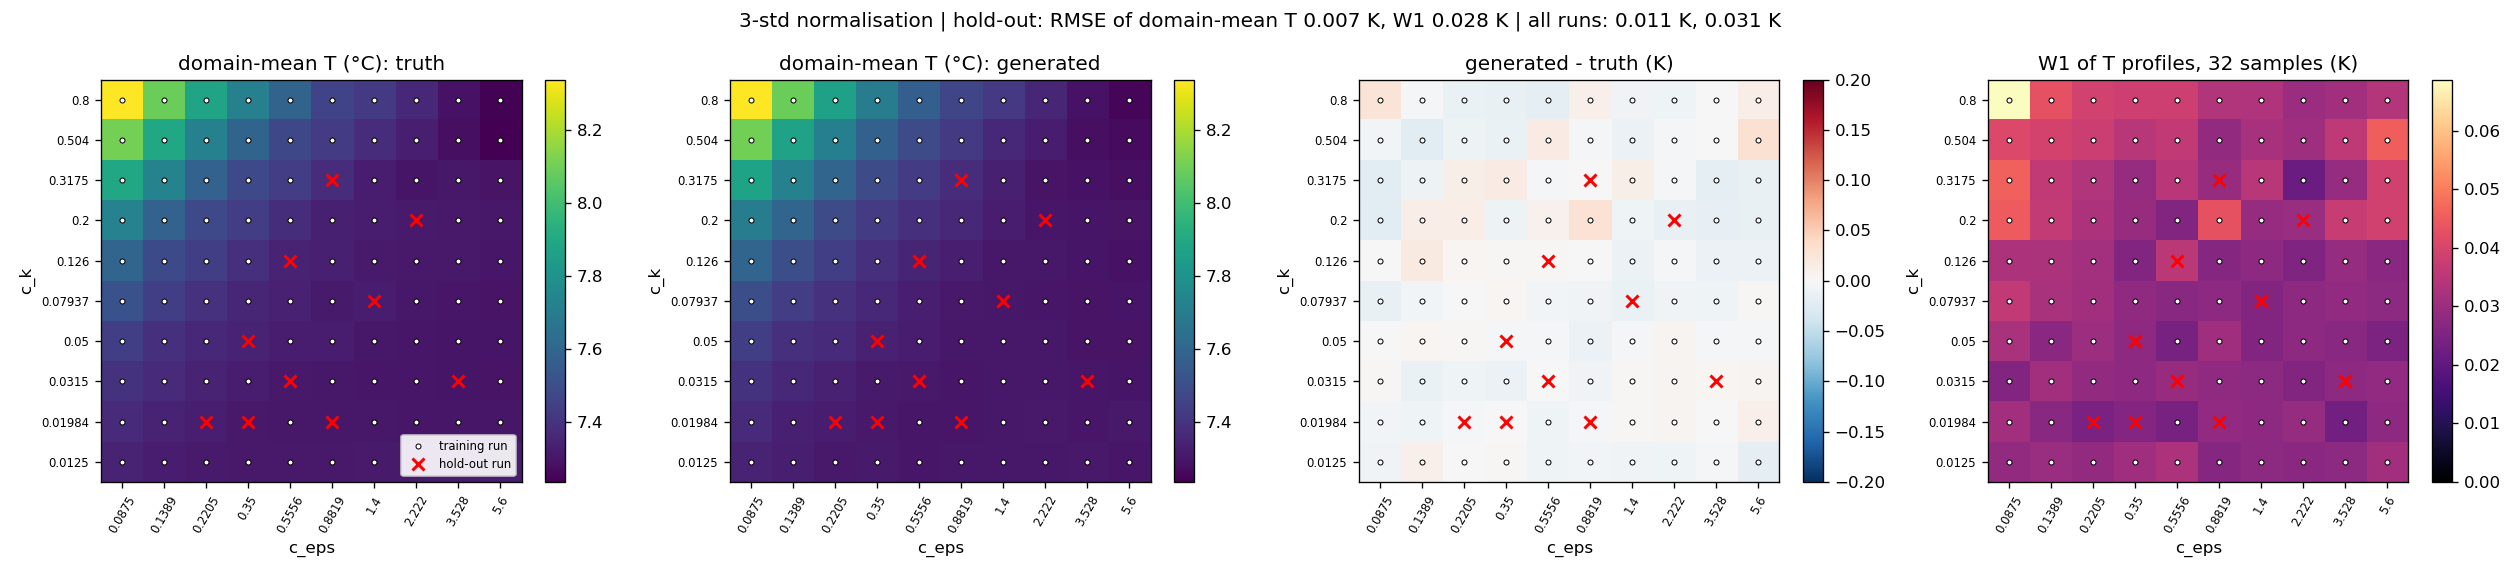
\includegraphics[width=\textwidth]{../fs_scattered_vml_3std/eval/grid_maps.png}
\caption{Over the parameter grid: domain-mean $T$ of the truth and of the generated states, their difference, and $W_1$ of the profile distribution. White dots: training runs; red crosses: held-out runs.}
\end{subfigure}\\[4pt]
\begin{subfigure}[b]{\textwidth}\centering
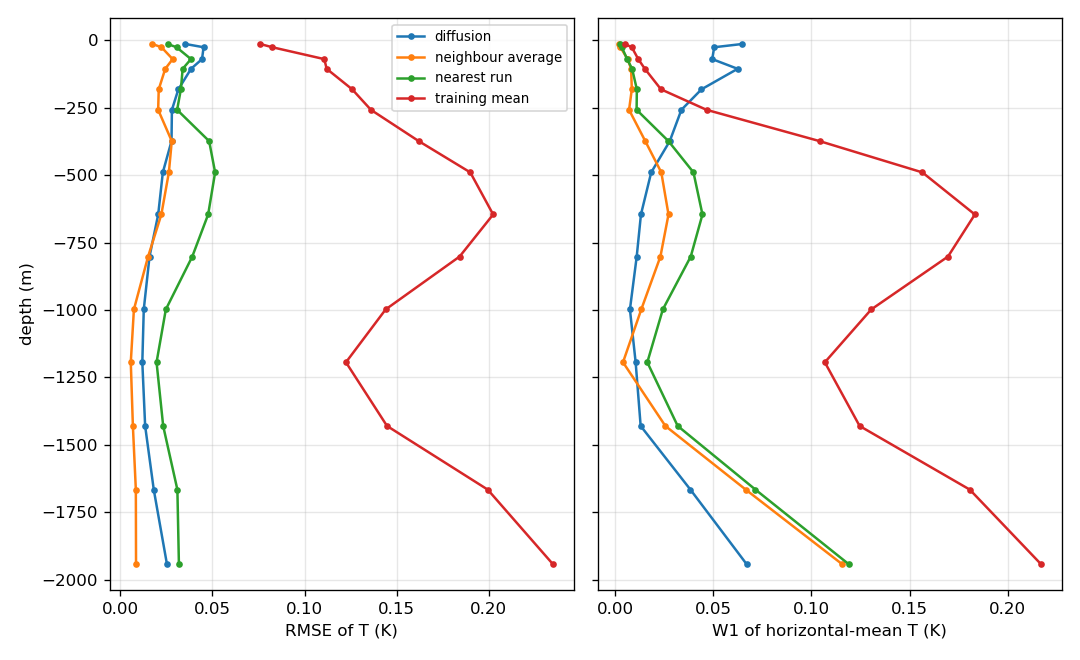
\includegraphics[width=0.62\textwidth]{../fs_scattered_vml_3std/eval/profiles.png}
\caption{RMSE (left) and $W_1$ (right) by depth, mean over the held-out runs.}
\end{subfigure}
\caption{Scattered split (10 interior held-out runs), 32 samples per run.}
\label{fig:scat}
\end{figure}

\begin{figure}[!htb]
\centering
\begin{subfigure}[b]{\textwidth}\centering
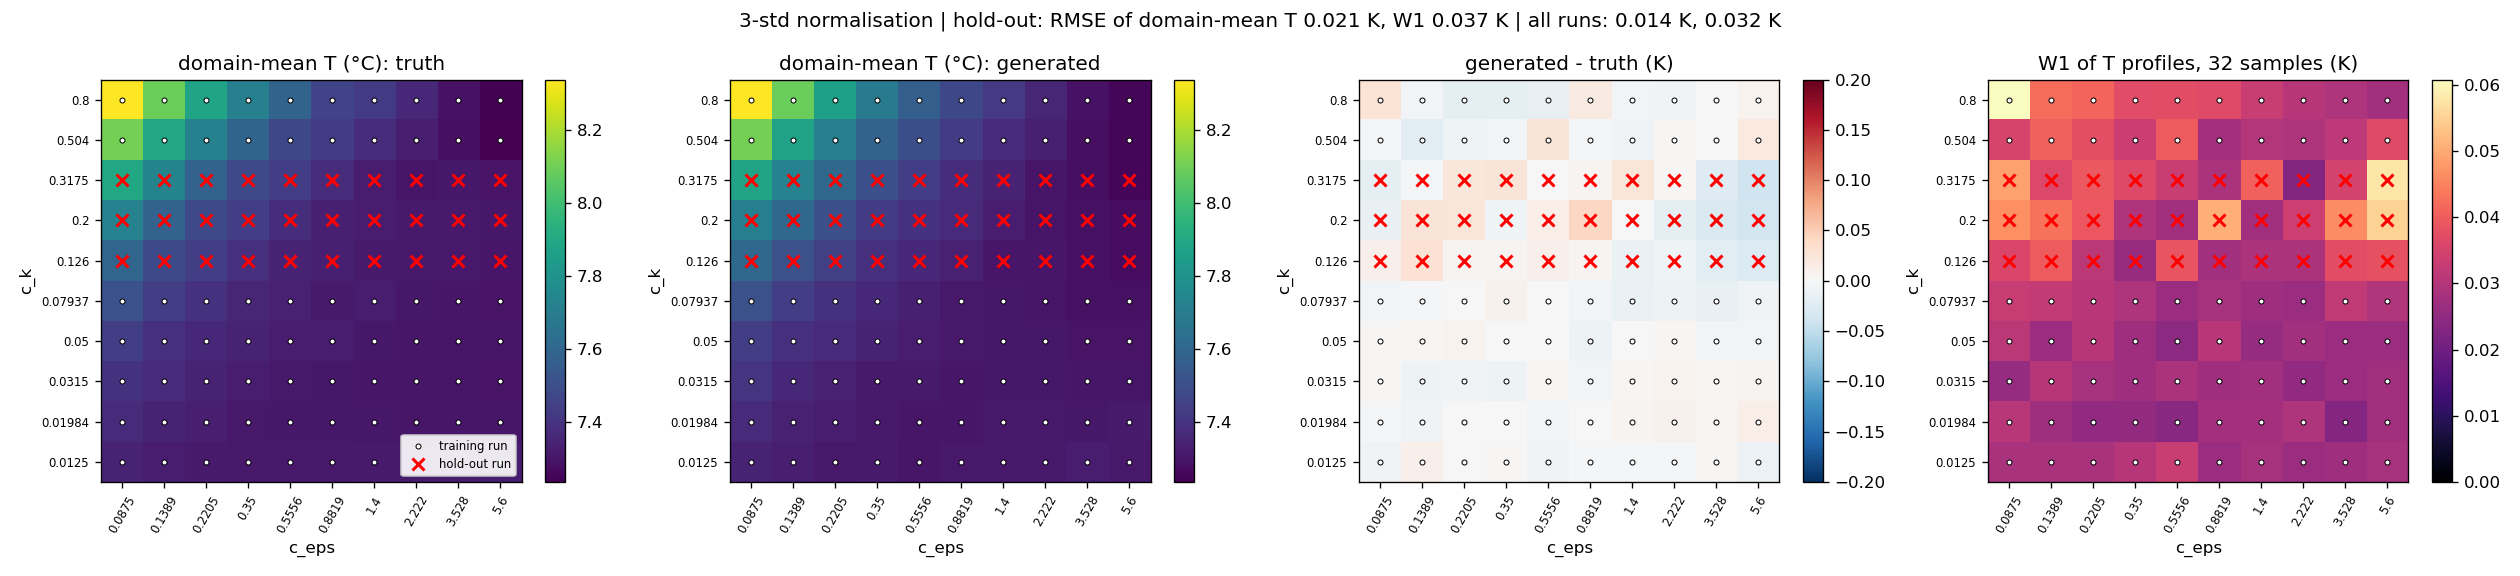
\includegraphics[width=\textwidth]{../fs_band3_vml_3std/eval/grid_maps.png}
\caption{Over the parameter grid: domain-mean $T$ of the truth and of the generated states, their difference, and $W_1$ of the profile distribution. White dots: training runs; red crosses: held-out runs.}
\end{subfigure}\\[4pt]
\begin{subfigure}[b]{\textwidth}\centering
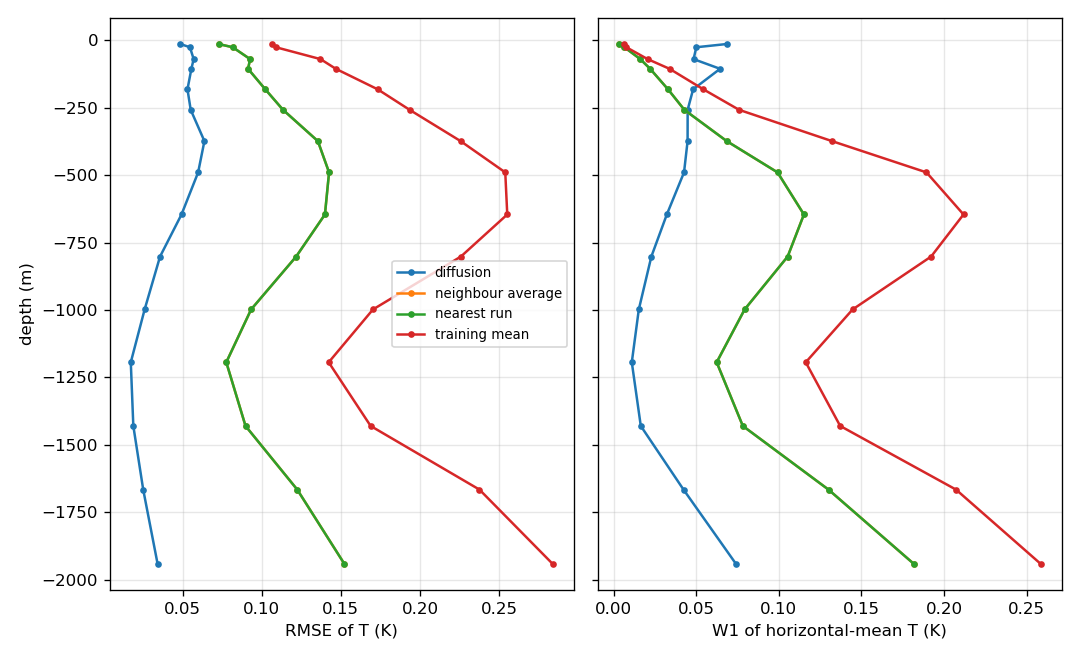
\includegraphics[width=0.62\textwidth]{../fs_band3_vml_3std/eval/profiles.png}
\caption{RMSE (left) and $W_1$ (right) by depth, mean over the held-out runs.}
\end{subfigure}
\caption{Band of three rows ($c_k$ = 0.126, 0.2, 0.3175 held out), 32 samples per run.}
\label{fig:band}
\end{figure}

\begin{figure}[!htb]
\centering
\begin{subfigure}[b]{\textwidth}\centering
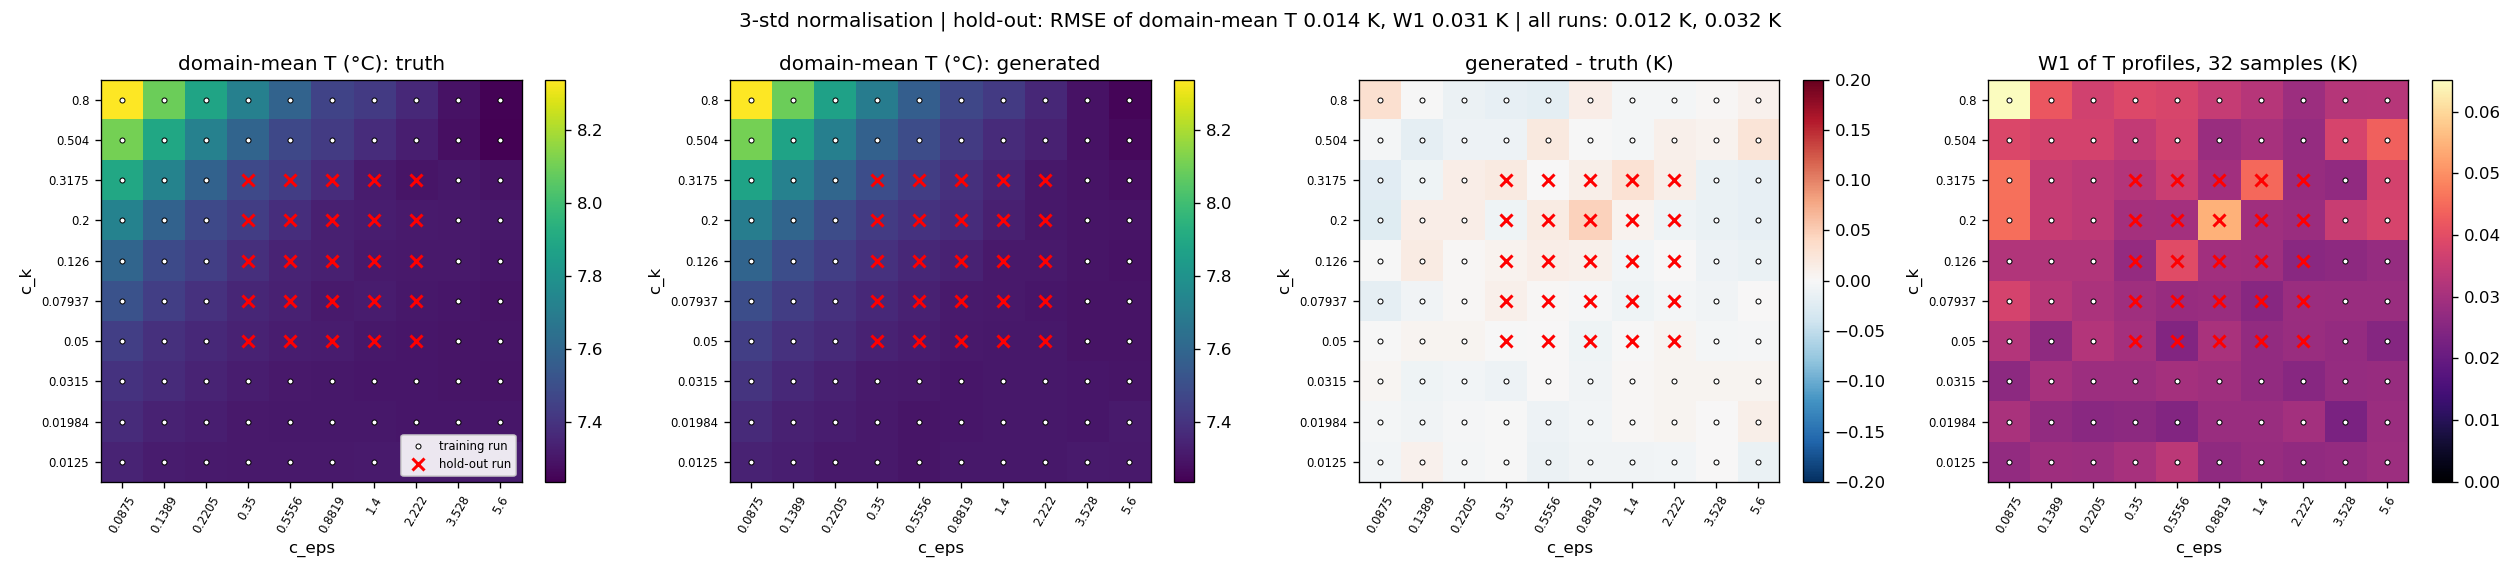
\includegraphics[width=\textwidth]{../fs_block5_vml_3std/eval/grid_maps.png}
\caption{Over the parameter grid: domain-mean $T$ of the truth and of the generated states, their difference, and $W_1$ of the profile distribution. White dots: training runs; red crosses: held-out runs.}
\end{subfigure}\\[4pt]
\begin{subfigure}[b]{\textwidth}\centering
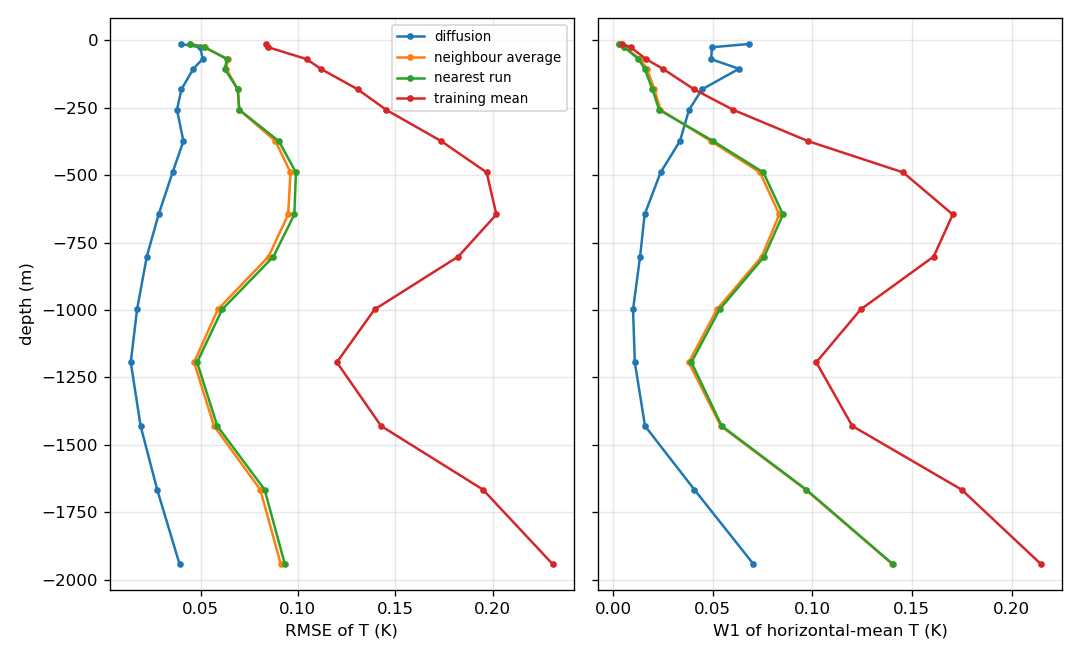
\includegraphics[width=0.62\textwidth]{../fs_block5_vml_3std/eval/profiles.png}
\caption{RMSE (left) and $W_1$ (right) by depth, mean over the held-out runs.}
\end{subfigure}
\caption{Centre $5\times5$ block held out (25 runs; training on the 75 outer runs), 32 samples per run.}
\label{fig:block5}
\end{figure}

\begin{figure}[!htb]
\centering
\begin{subfigure}[b]{\textwidth}\centering
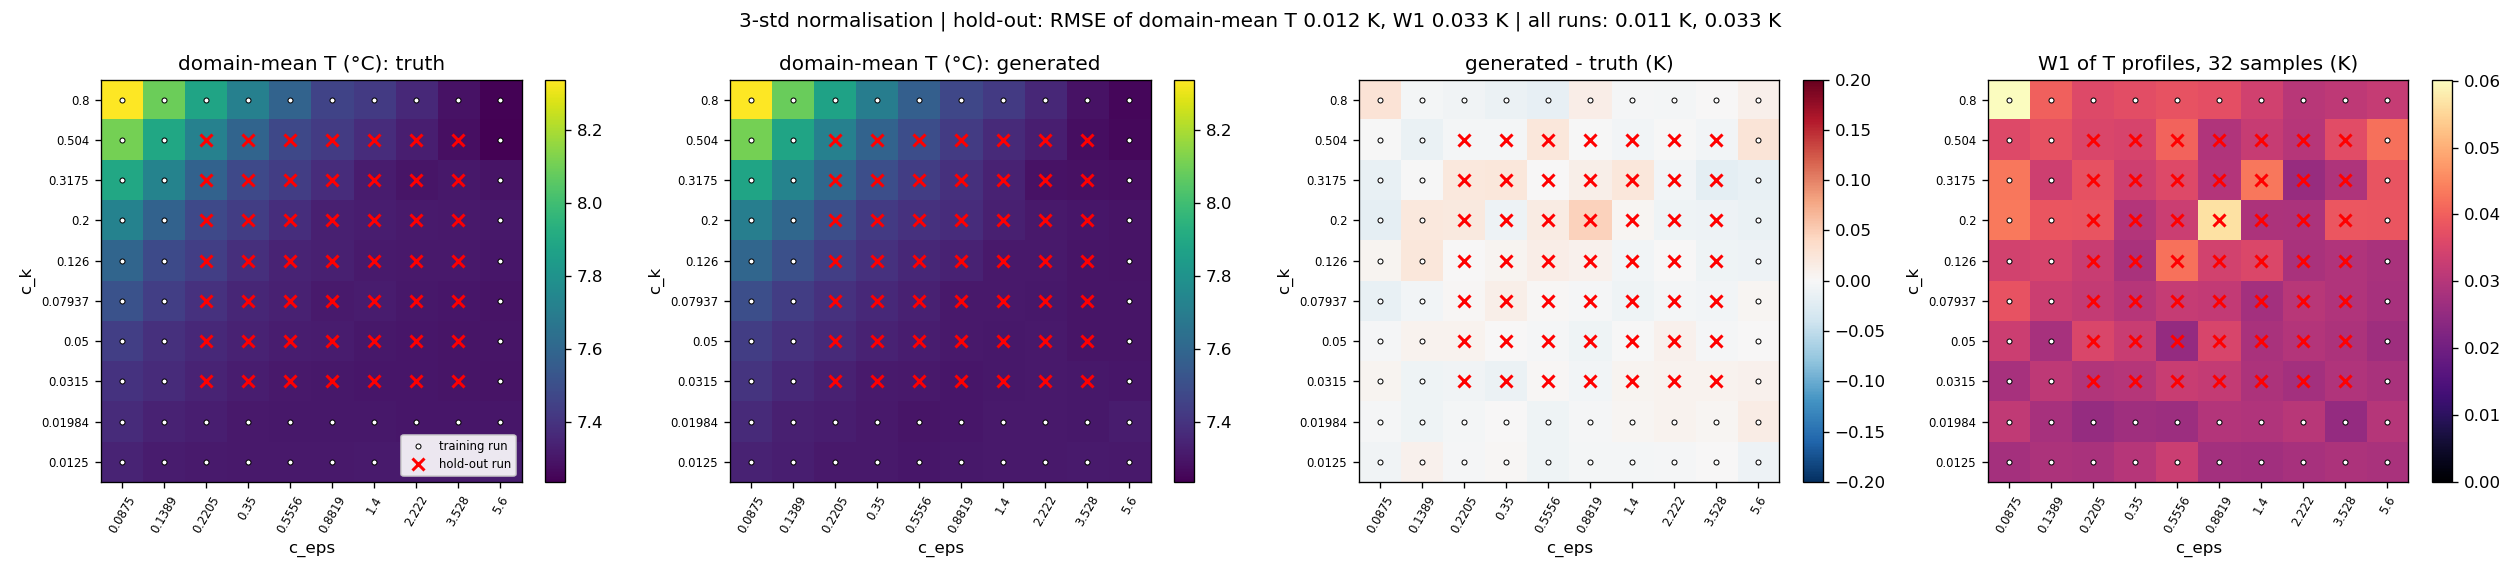
\includegraphics[width=\textwidth]{../fs_block_vml_3std/eval/grid_maps.png}
\caption{Over the parameter grid: domain-mean $T$ of the truth and of the generated states, their difference, and $W_1$ of the profile distribution. White dots: training runs; red crosses: held-out runs.}
\end{subfigure}\\[4pt]
\begin{subfigure}[b]{\textwidth}\centering
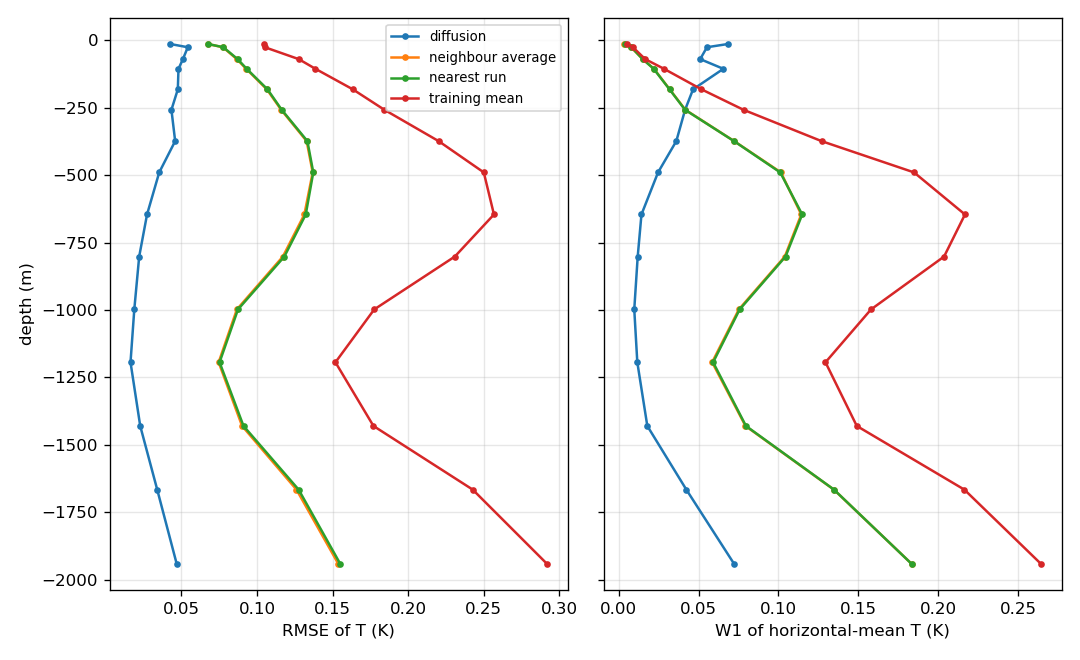
\includegraphics[width=0.62\textwidth]{../fs_block_vml_3std/eval/profiles.png}
\caption{RMSE (left) and $W_1$ (right) by depth, mean over the held-out runs.}
\end{subfigure}
\caption{Centre $7\times7$ block held out (49 runs; training on the 51 edge runs), 32 samples per run.}
\label{fig:block}
\end{figure}

\begin{figure}[!htb]
\centering
\begin{subfigure}[b]{\textwidth}\centering
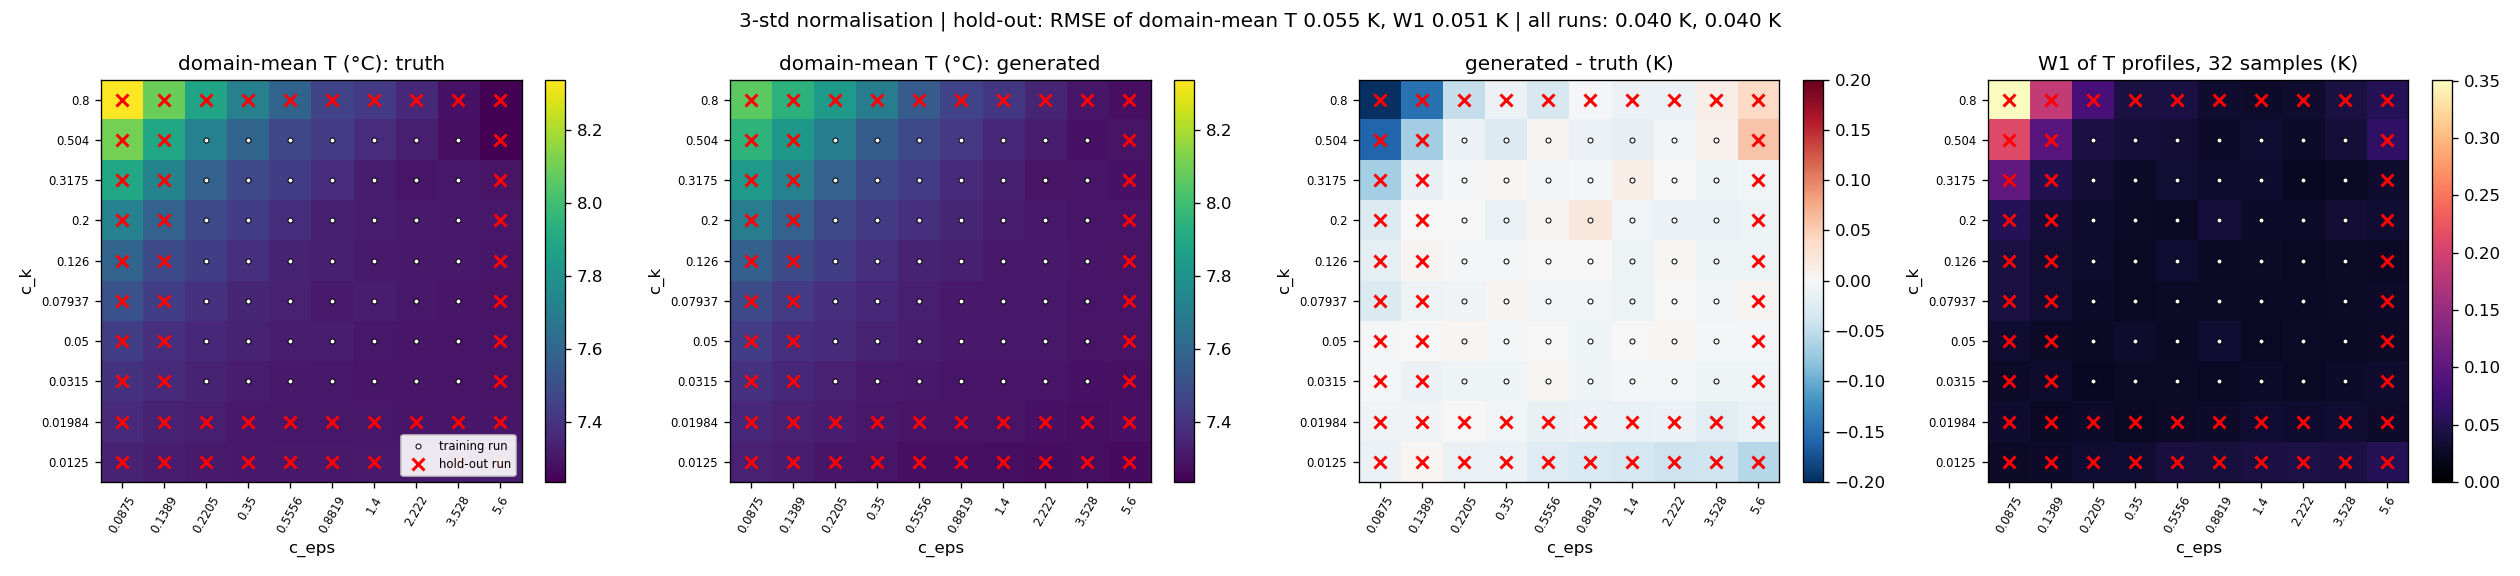
\includegraphics[width=\textwidth]{../fs_ring_vml_3std/eval/grid_maps.png}
\caption{Over the parameter grid: domain-mean $T$ of the truth and of the generated states, their difference, and $W_1$ of the profile distribution. White dots: training runs; red crosses: held-out runs.}
\end{subfigure}\\[4pt]
\begin{subfigure}[b]{\textwidth}\centering
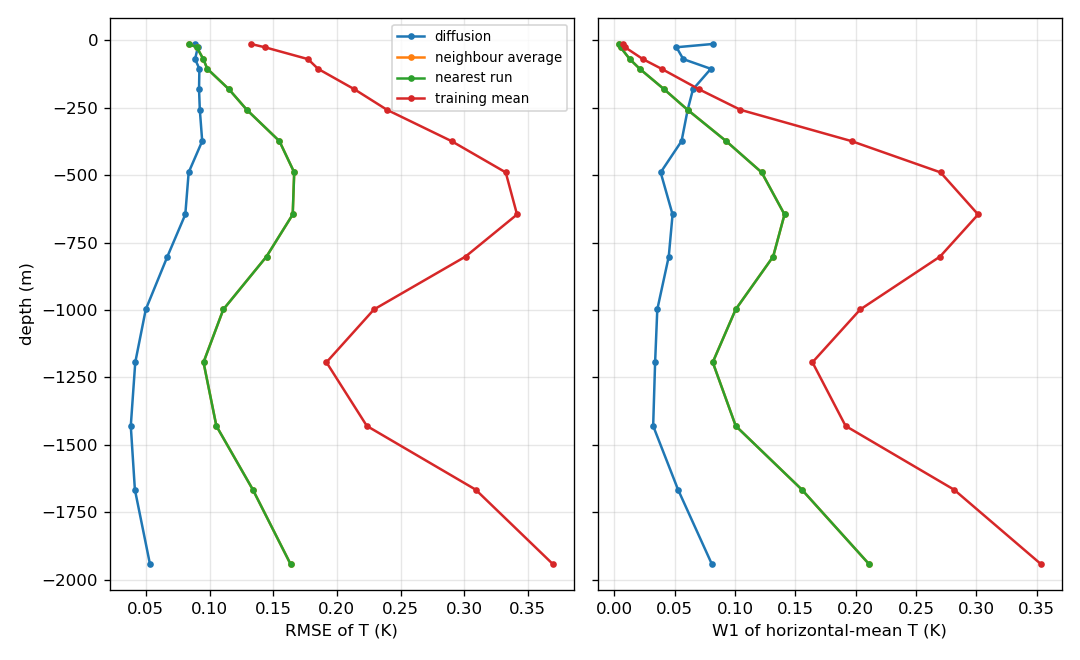
\includegraphics[width=0.62\textwidth]{../fs_ring_vml_3std/eval/profiles.png}
\caption{RMSE (left) and $W_1$ (right) by depth, mean over the held-out runs.}
\end{subfigure}
\caption{Outer 51 held out (training on the $7\times7$ centre), 32 samples per run.}
\label{fig:ring}
\end{figure}

\begin{figure}[!htb]
\centering
\begin{subfigure}[b]{\textwidth}\centering
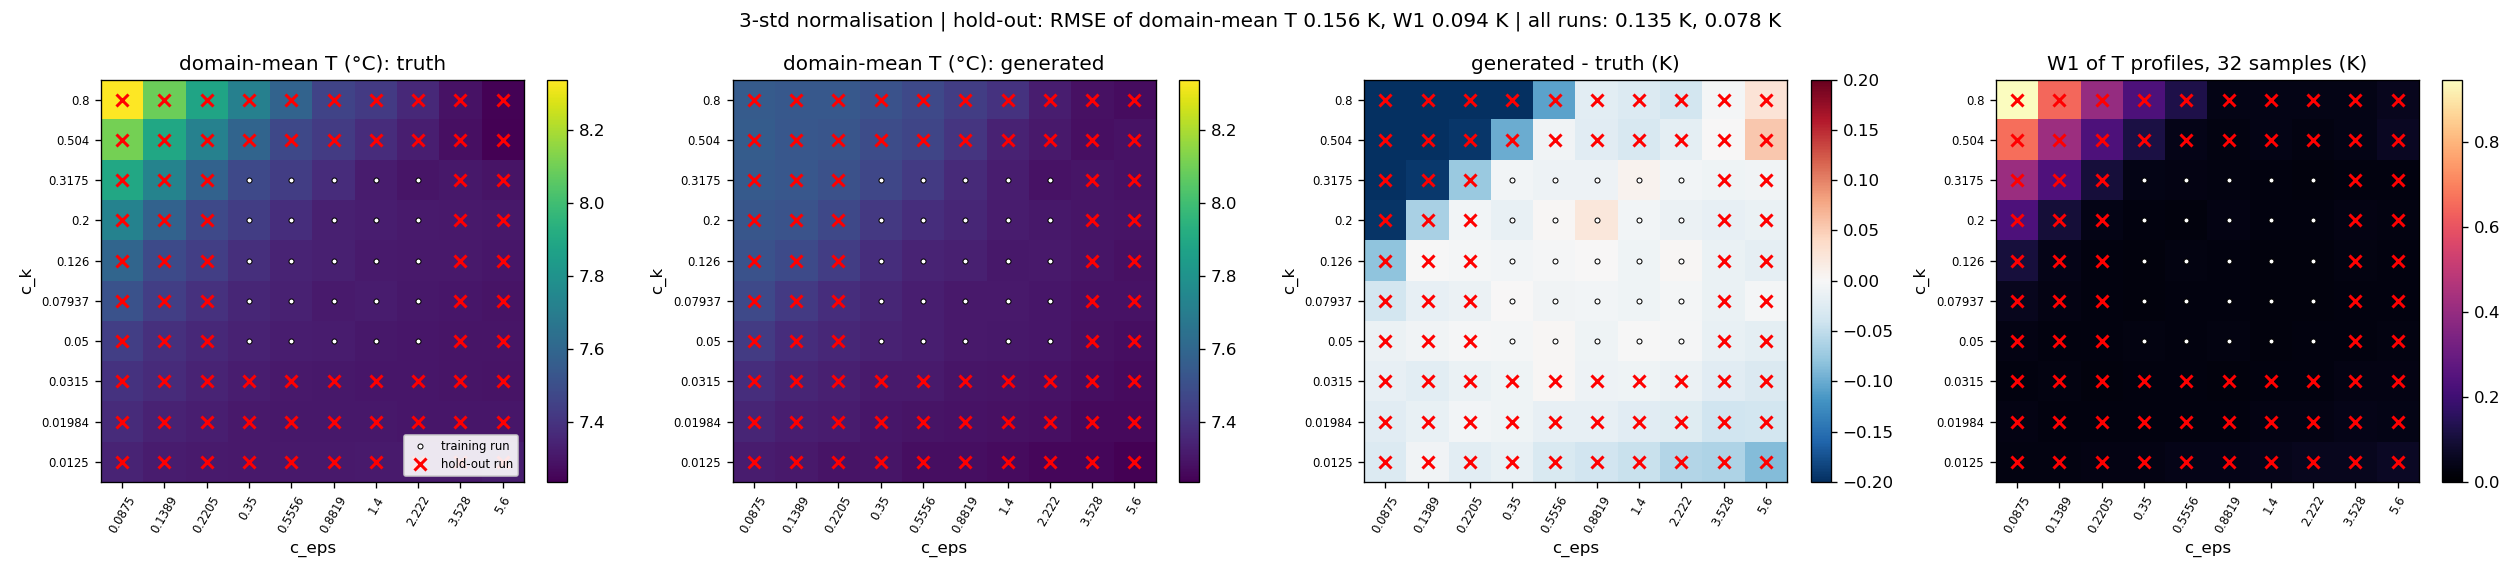
\includegraphics[width=\textwidth]{../fs_ring5_vml_3std/eval/grid_maps.png}
\caption{Over the parameter grid: domain-mean $T$ of the truth and of the generated states, their difference, and $W_1$ of the profile distribution. White dots: training runs; red crosses: held-out runs.}
\end{subfigure}\\[4pt]
\begin{subfigure}[b]{\textwidth}\centering
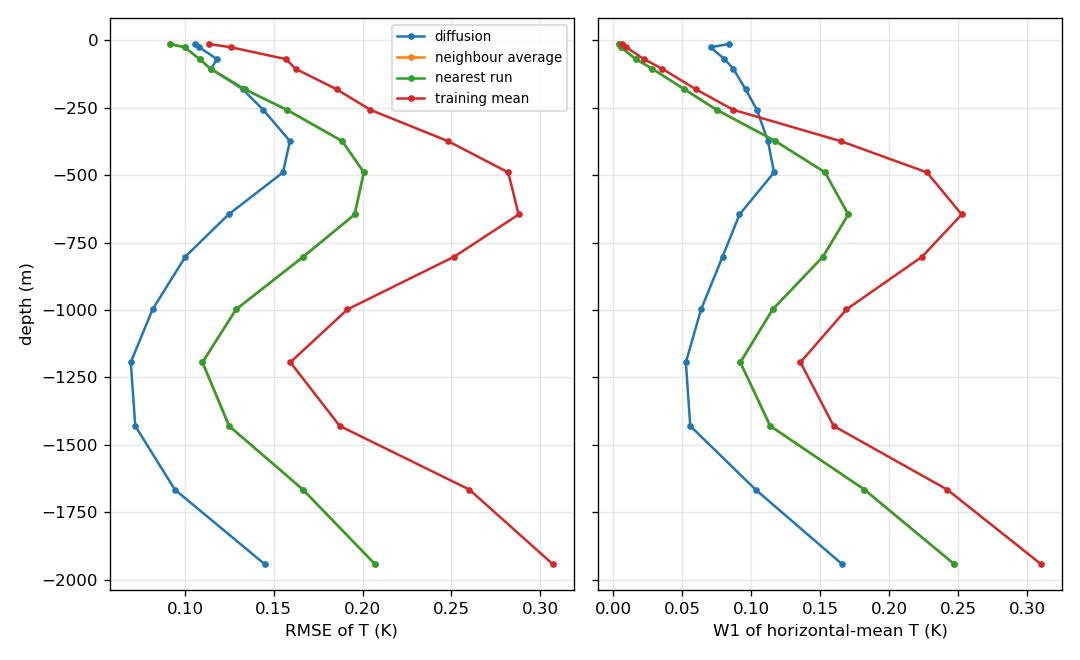
\includegraphics[width=0.62\textwidth]{../fs_ring5_vml_3std/eval/profiles.png}
\caption{RMSE (left) and $W_1$ (right) by depth, mean over the held-out runs.}
\end{subfigure}
\caption{Outer 75 held out (training on the $5\times5$ centre), 32 samples per run.}
\label{fig:ring5}
\end{figure}

\begin{figure}[!htb]
\centering
\begin{subfigure}[b]{\textwidth}\centering
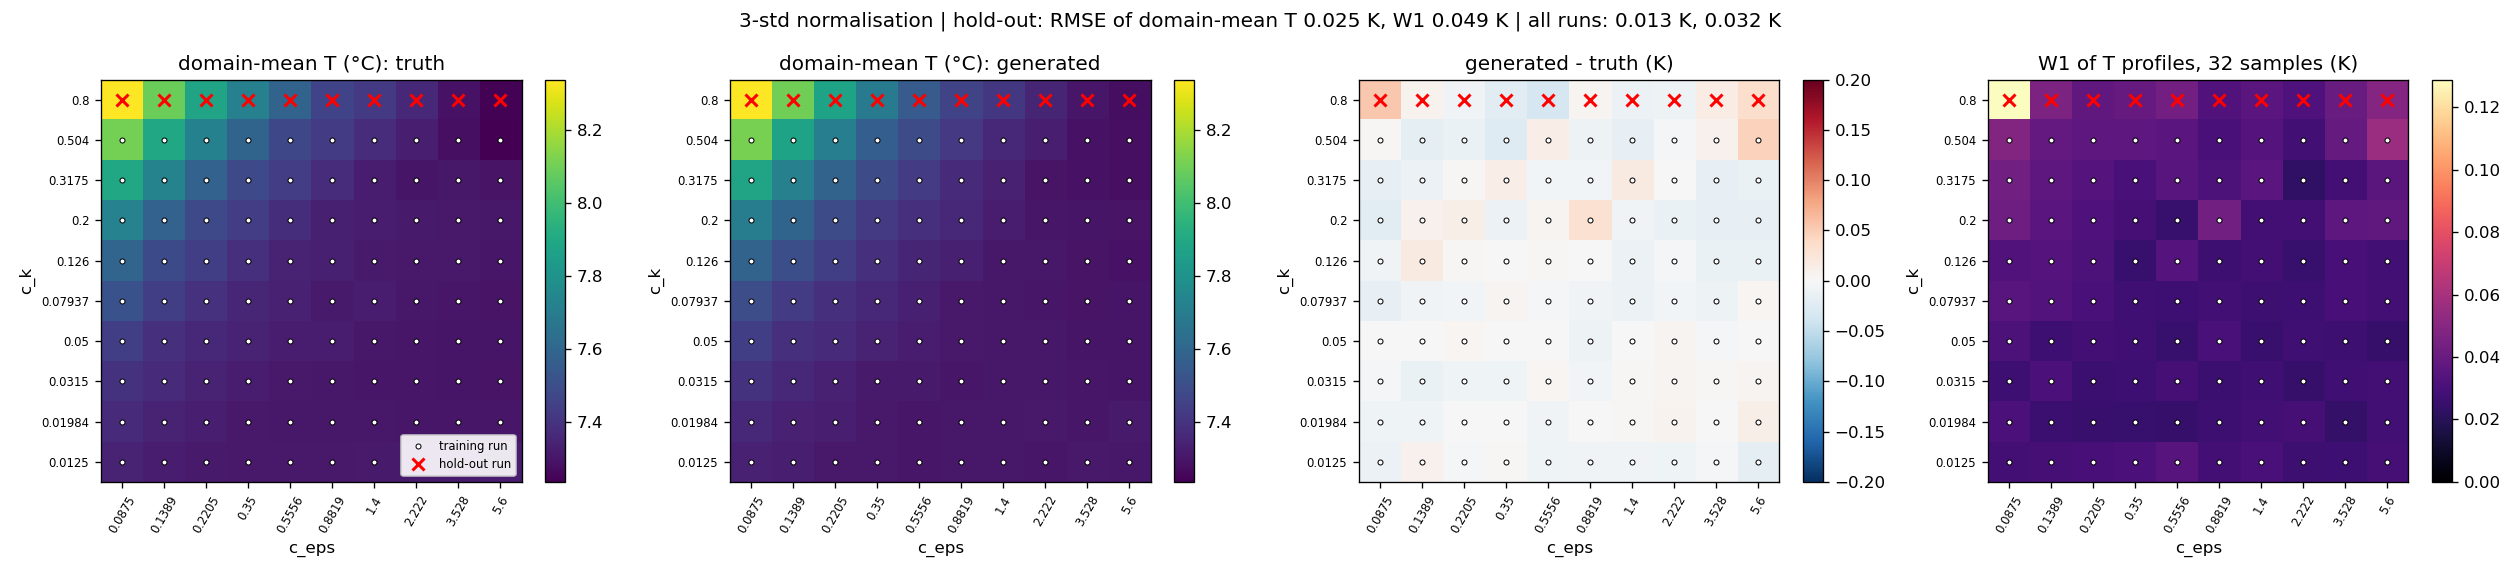
\includegraphics[width=\textwidth]{../fs_top_vml_3std/eval/grid_maps.png}
\caption{Over the parameter grid: domain-mean $T$ of the truth and of the generated states, their difference, and $W_1$ of the profile distribution. White dots: training runs; red crosses: held-out runs.}
\end{subfigure}\\[4pt]
\begin{subfigure}[b]{\textwidth}\centering
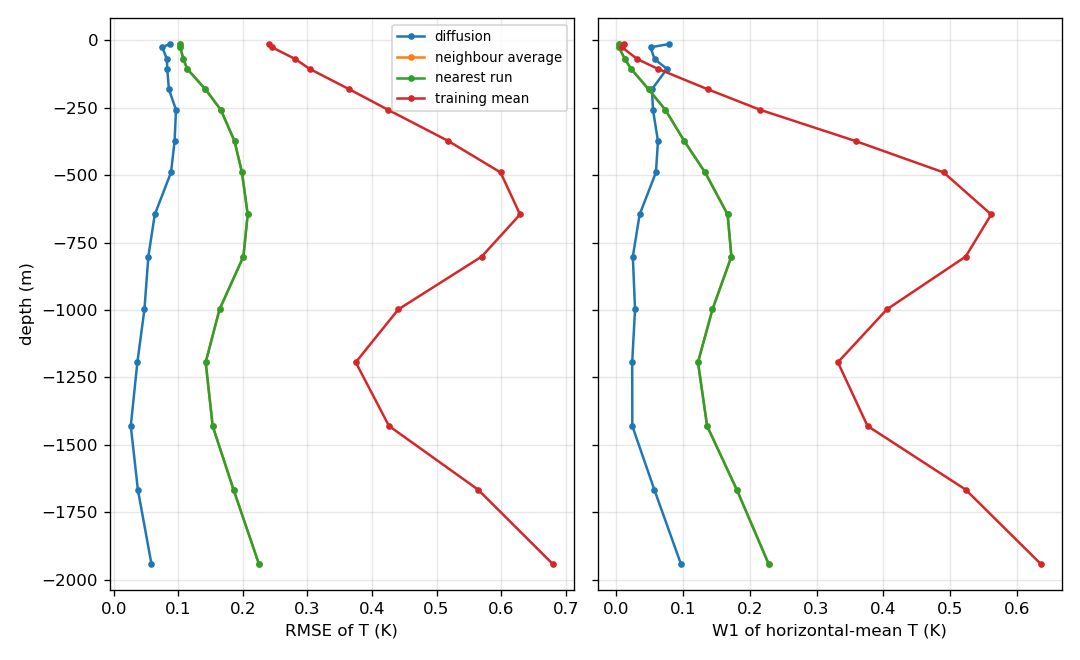
\includegraphics[width=0.62\textwidth]{../fs_top_vml_3std/eval/profiles.png}
\caption{RMSE (left) and $W_1$ (right) by depth, mean over the held-out runs.}
\end{subfigure}
\caption{Top row held out ($c_k$ = 0.8, 10 runs), 32 samples per run.}
\label{fig:top}
\end{figure}

\begin{figure}[!htb]
\centering
\begin{subfigure}[b]{\textwidth}\centering
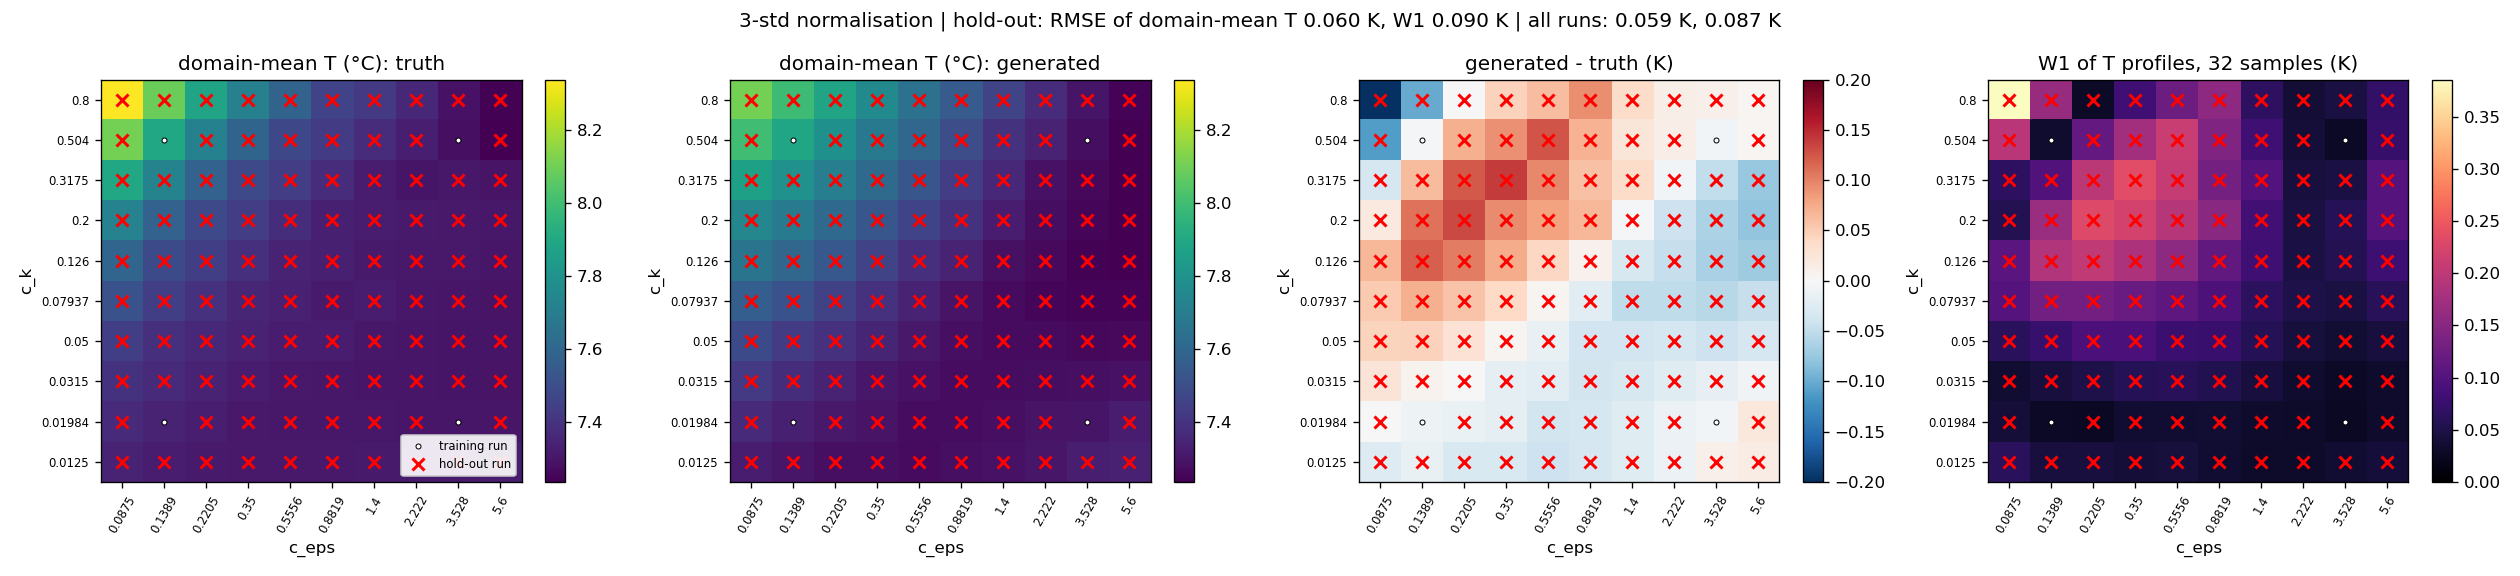
\includegraphics[width=\textwidth]{../fs_four_vml_3std/eval/grid_maps.png}
\caption{Over the parameter grid: domain-mean $T$ of the truth and of the generated states, their difference, and $W_1$ of the profile distribution. White dots: training runs; red crosses: held-out runs.}
\end{subfigure}\\[4pt]
\begin{subfigure}[b]{\textwidth}\centering
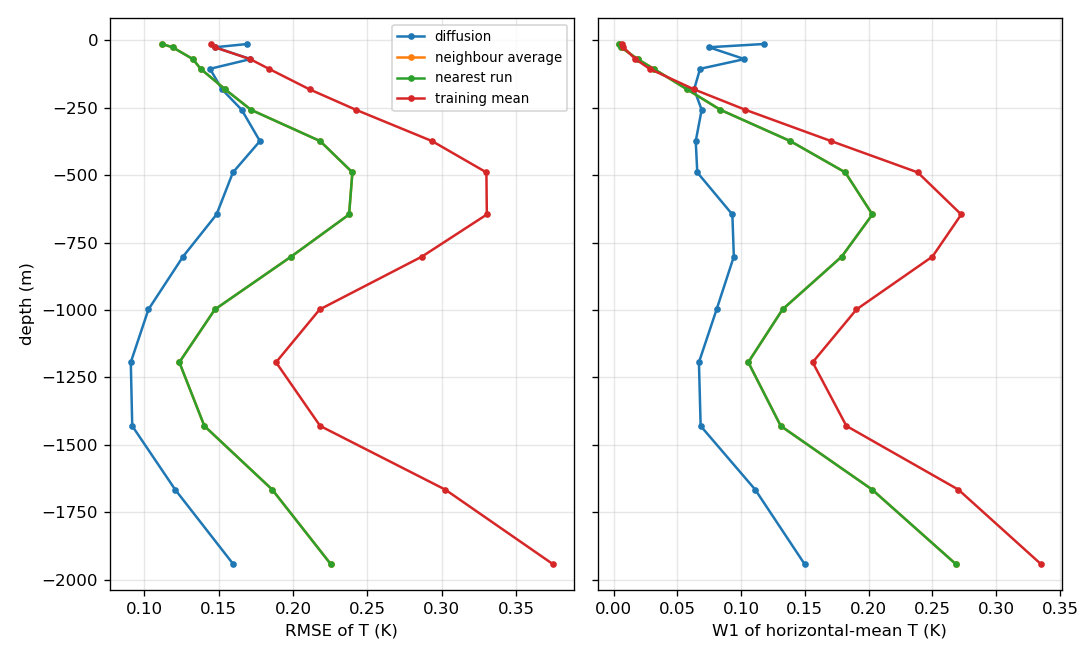
\includegraphics[width=0.62\textwidth]{../fs_four_vml_3std/eval/profiles.png}
\caption{RMSE (left) and $W_1$ (right) by depth, mean over the held-out runs.}
\end{subfigure}
\caption{Four training runs, one step in from each corner (96 held out), 32 samples per run.}
\label{fig:four}
\end{figure}

\begin{figure}[!htb]
\centering
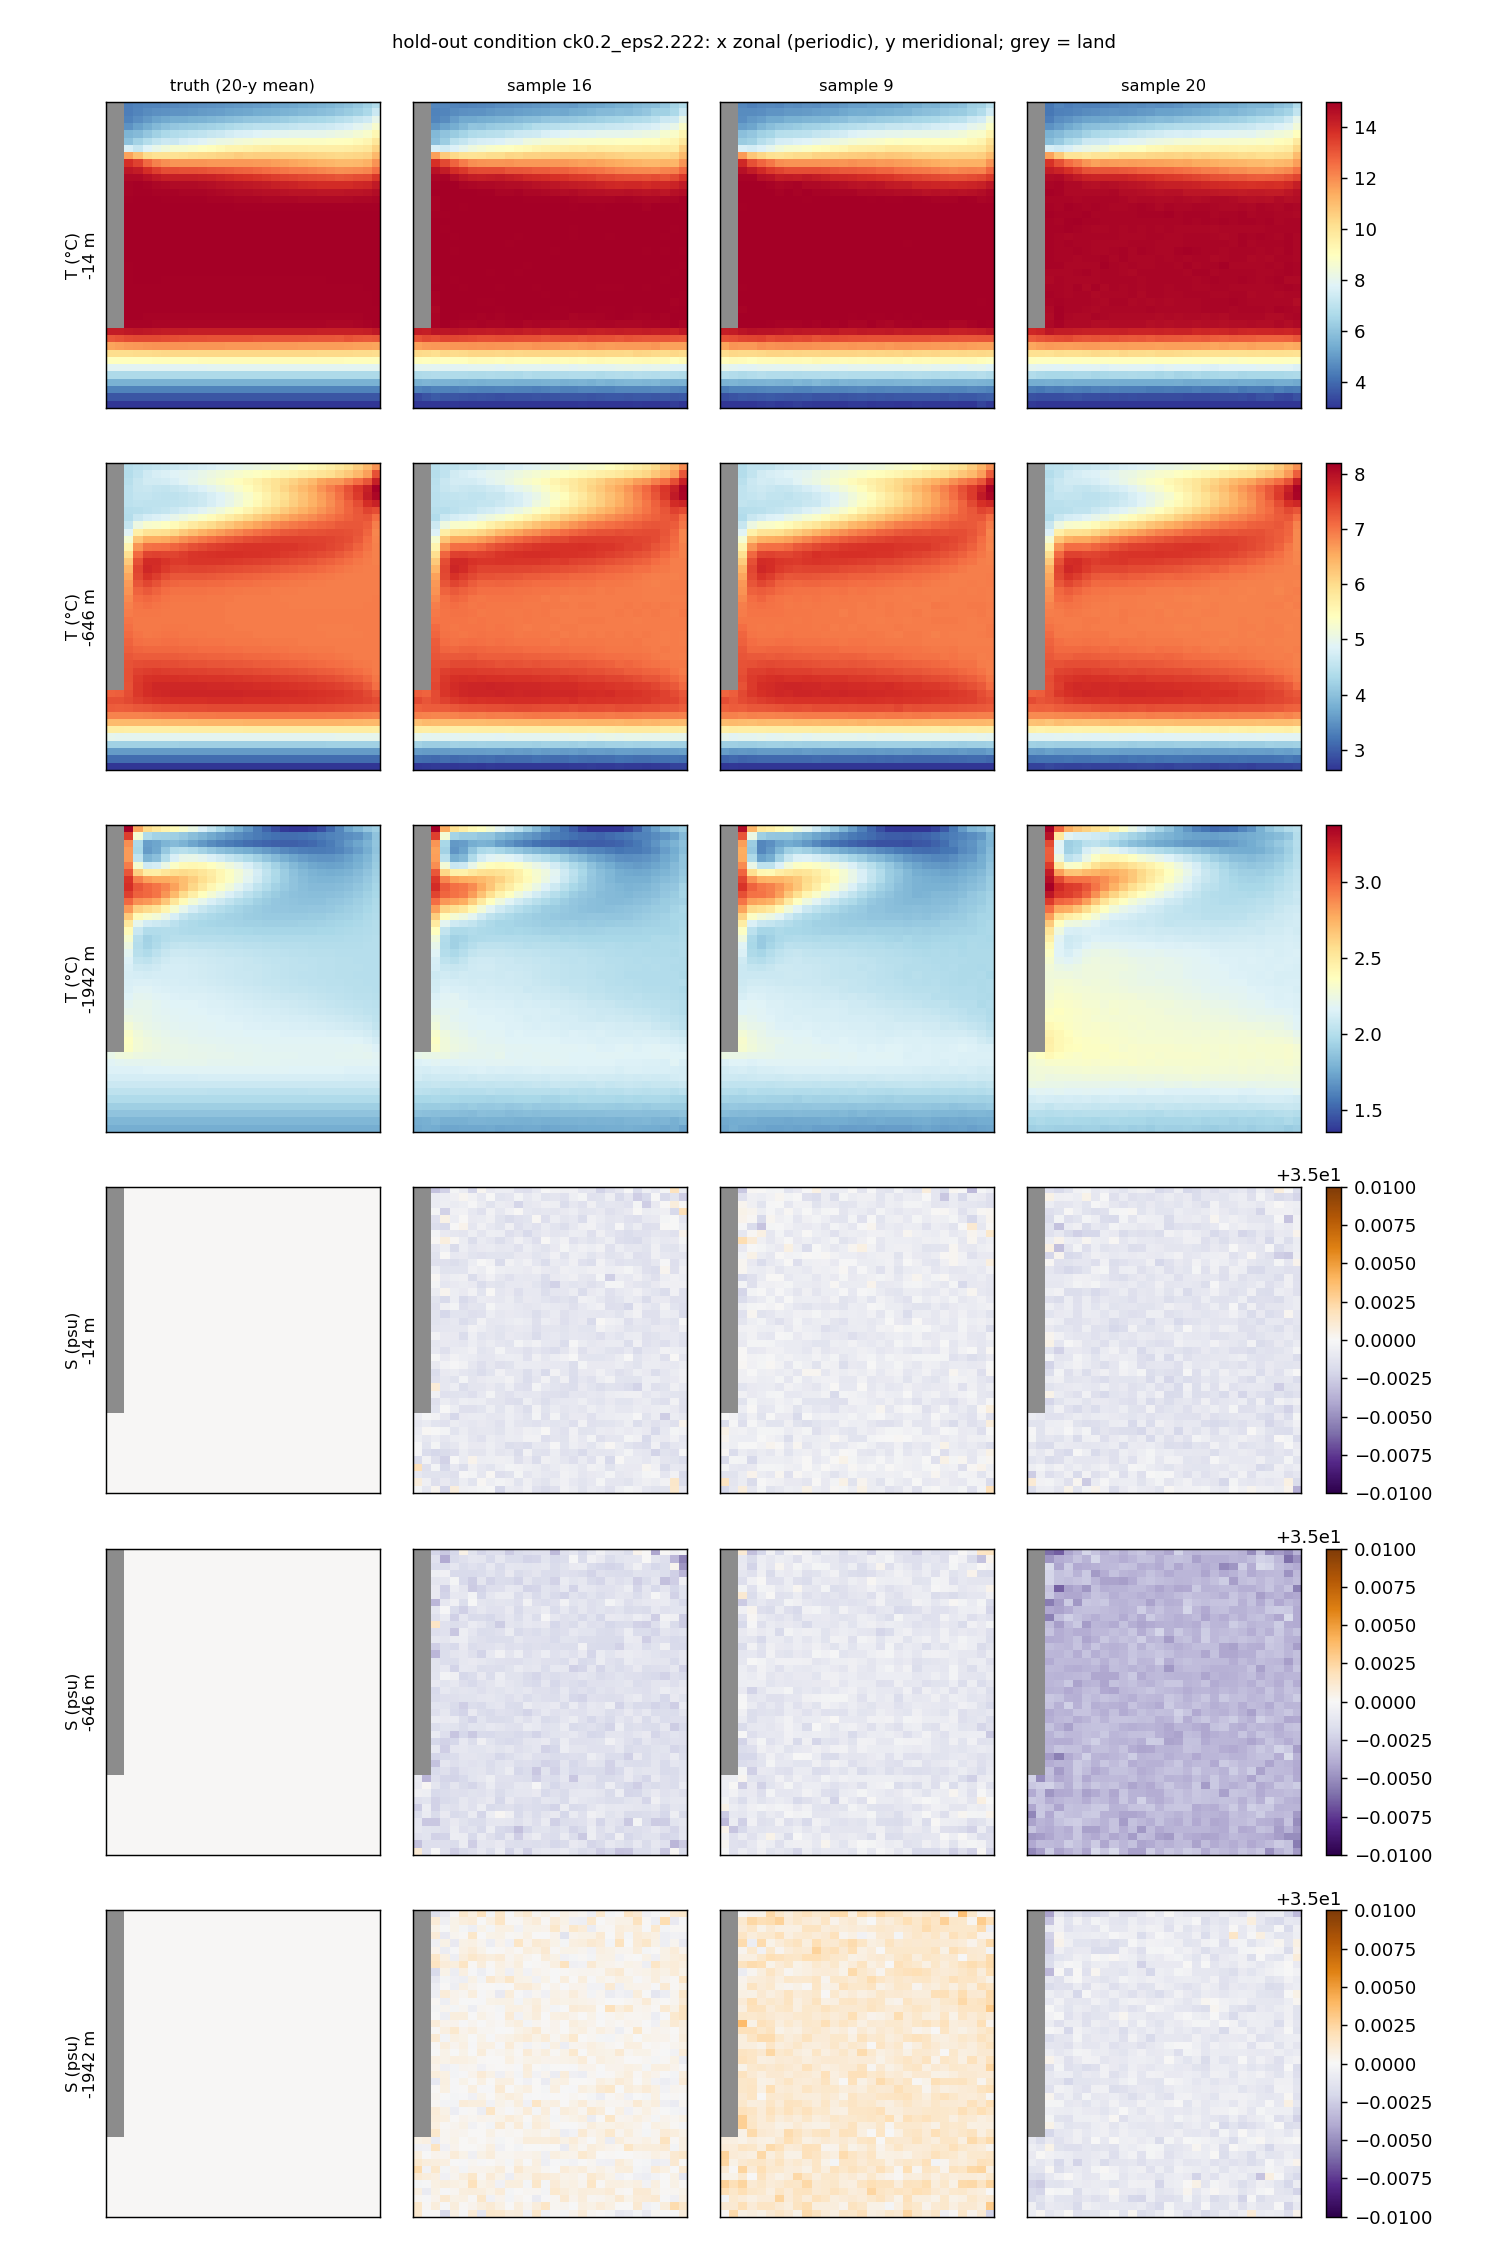
\includegraphics[width=0.9\textwidth]{../fs_scattered_vml_3std/samples_levels.png}
\caption{True 20-year mean state and three random samples of $T$ and $S$ at the surface, \SI{646}{m} and the bottom for one held-out condition of the scattered split (grey: land; $x$ zonal and periodic, $y$ meridional).}
\label{fig:samples}
\end{figure}

\begin{figure}[!htb]
\centering
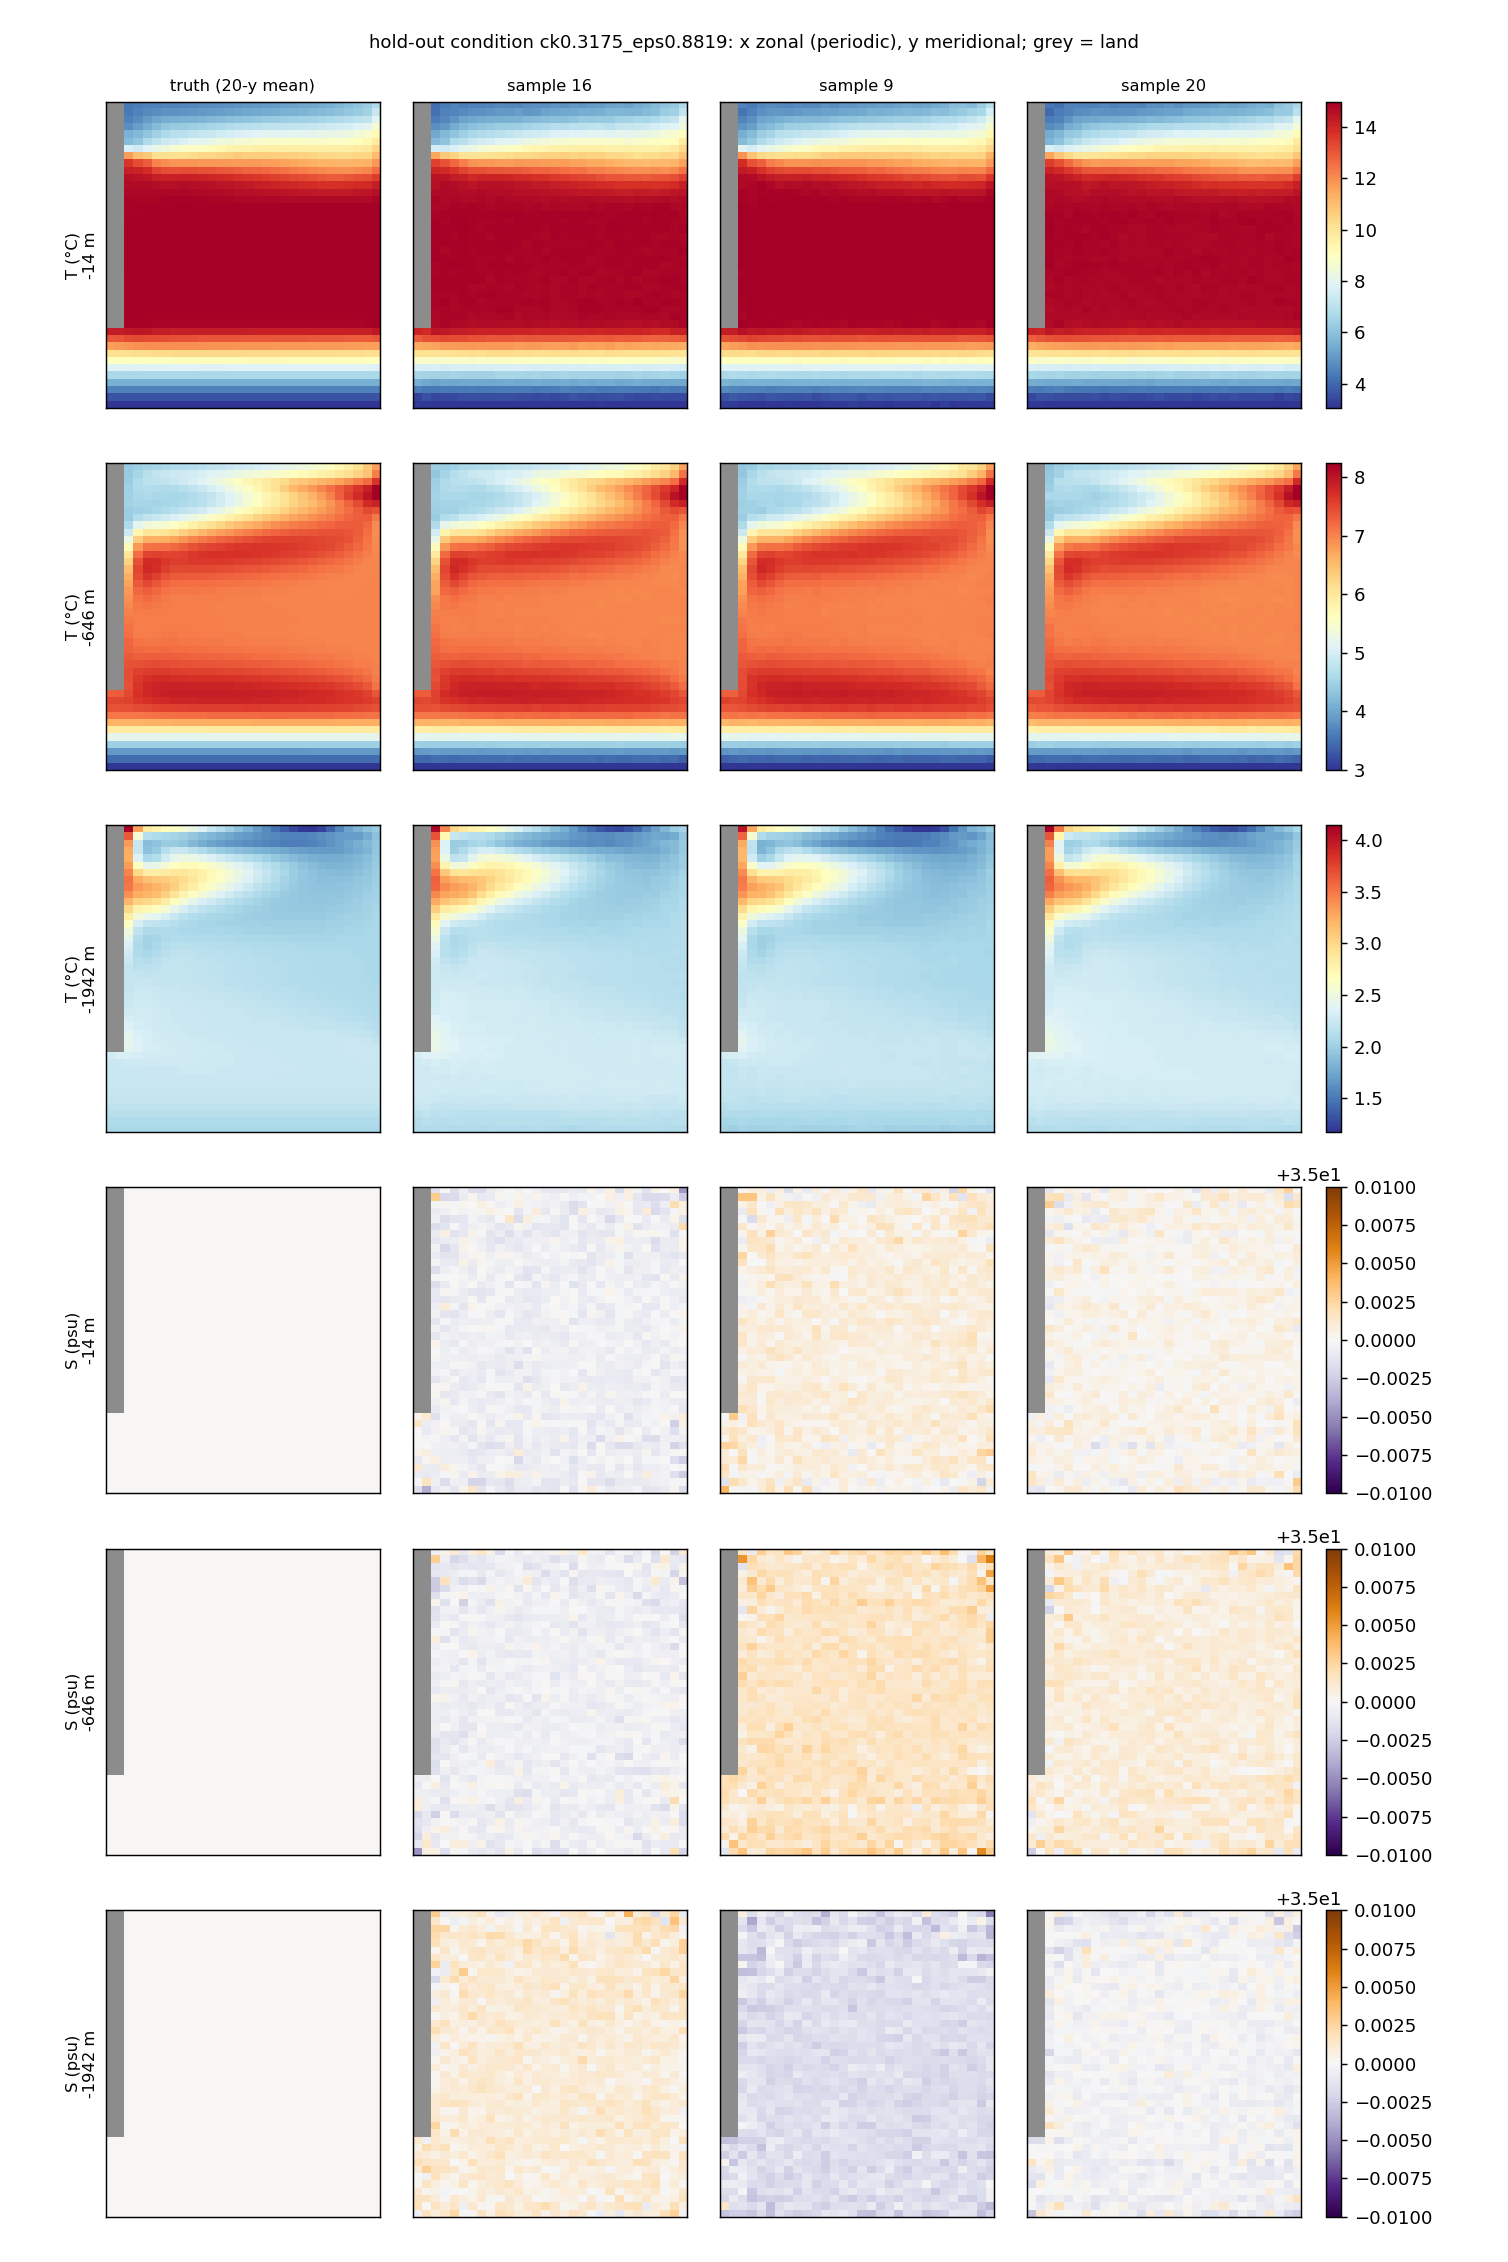
\includegraphics[width=0.9\textwidth]{../fs_band3_vml_3std/samples_levels.png}
\caption{True 20-year mean state and three random samples of $T$ and $S$ at the surface, \SI{646}{m} and the bottom for one held-out condition of the band split (grey: land; $x$ zonal and periodic, $y$ meridional).}
\label{fig:samples_band}
\end{figure}

\begin{figure}[!htb]
\centering
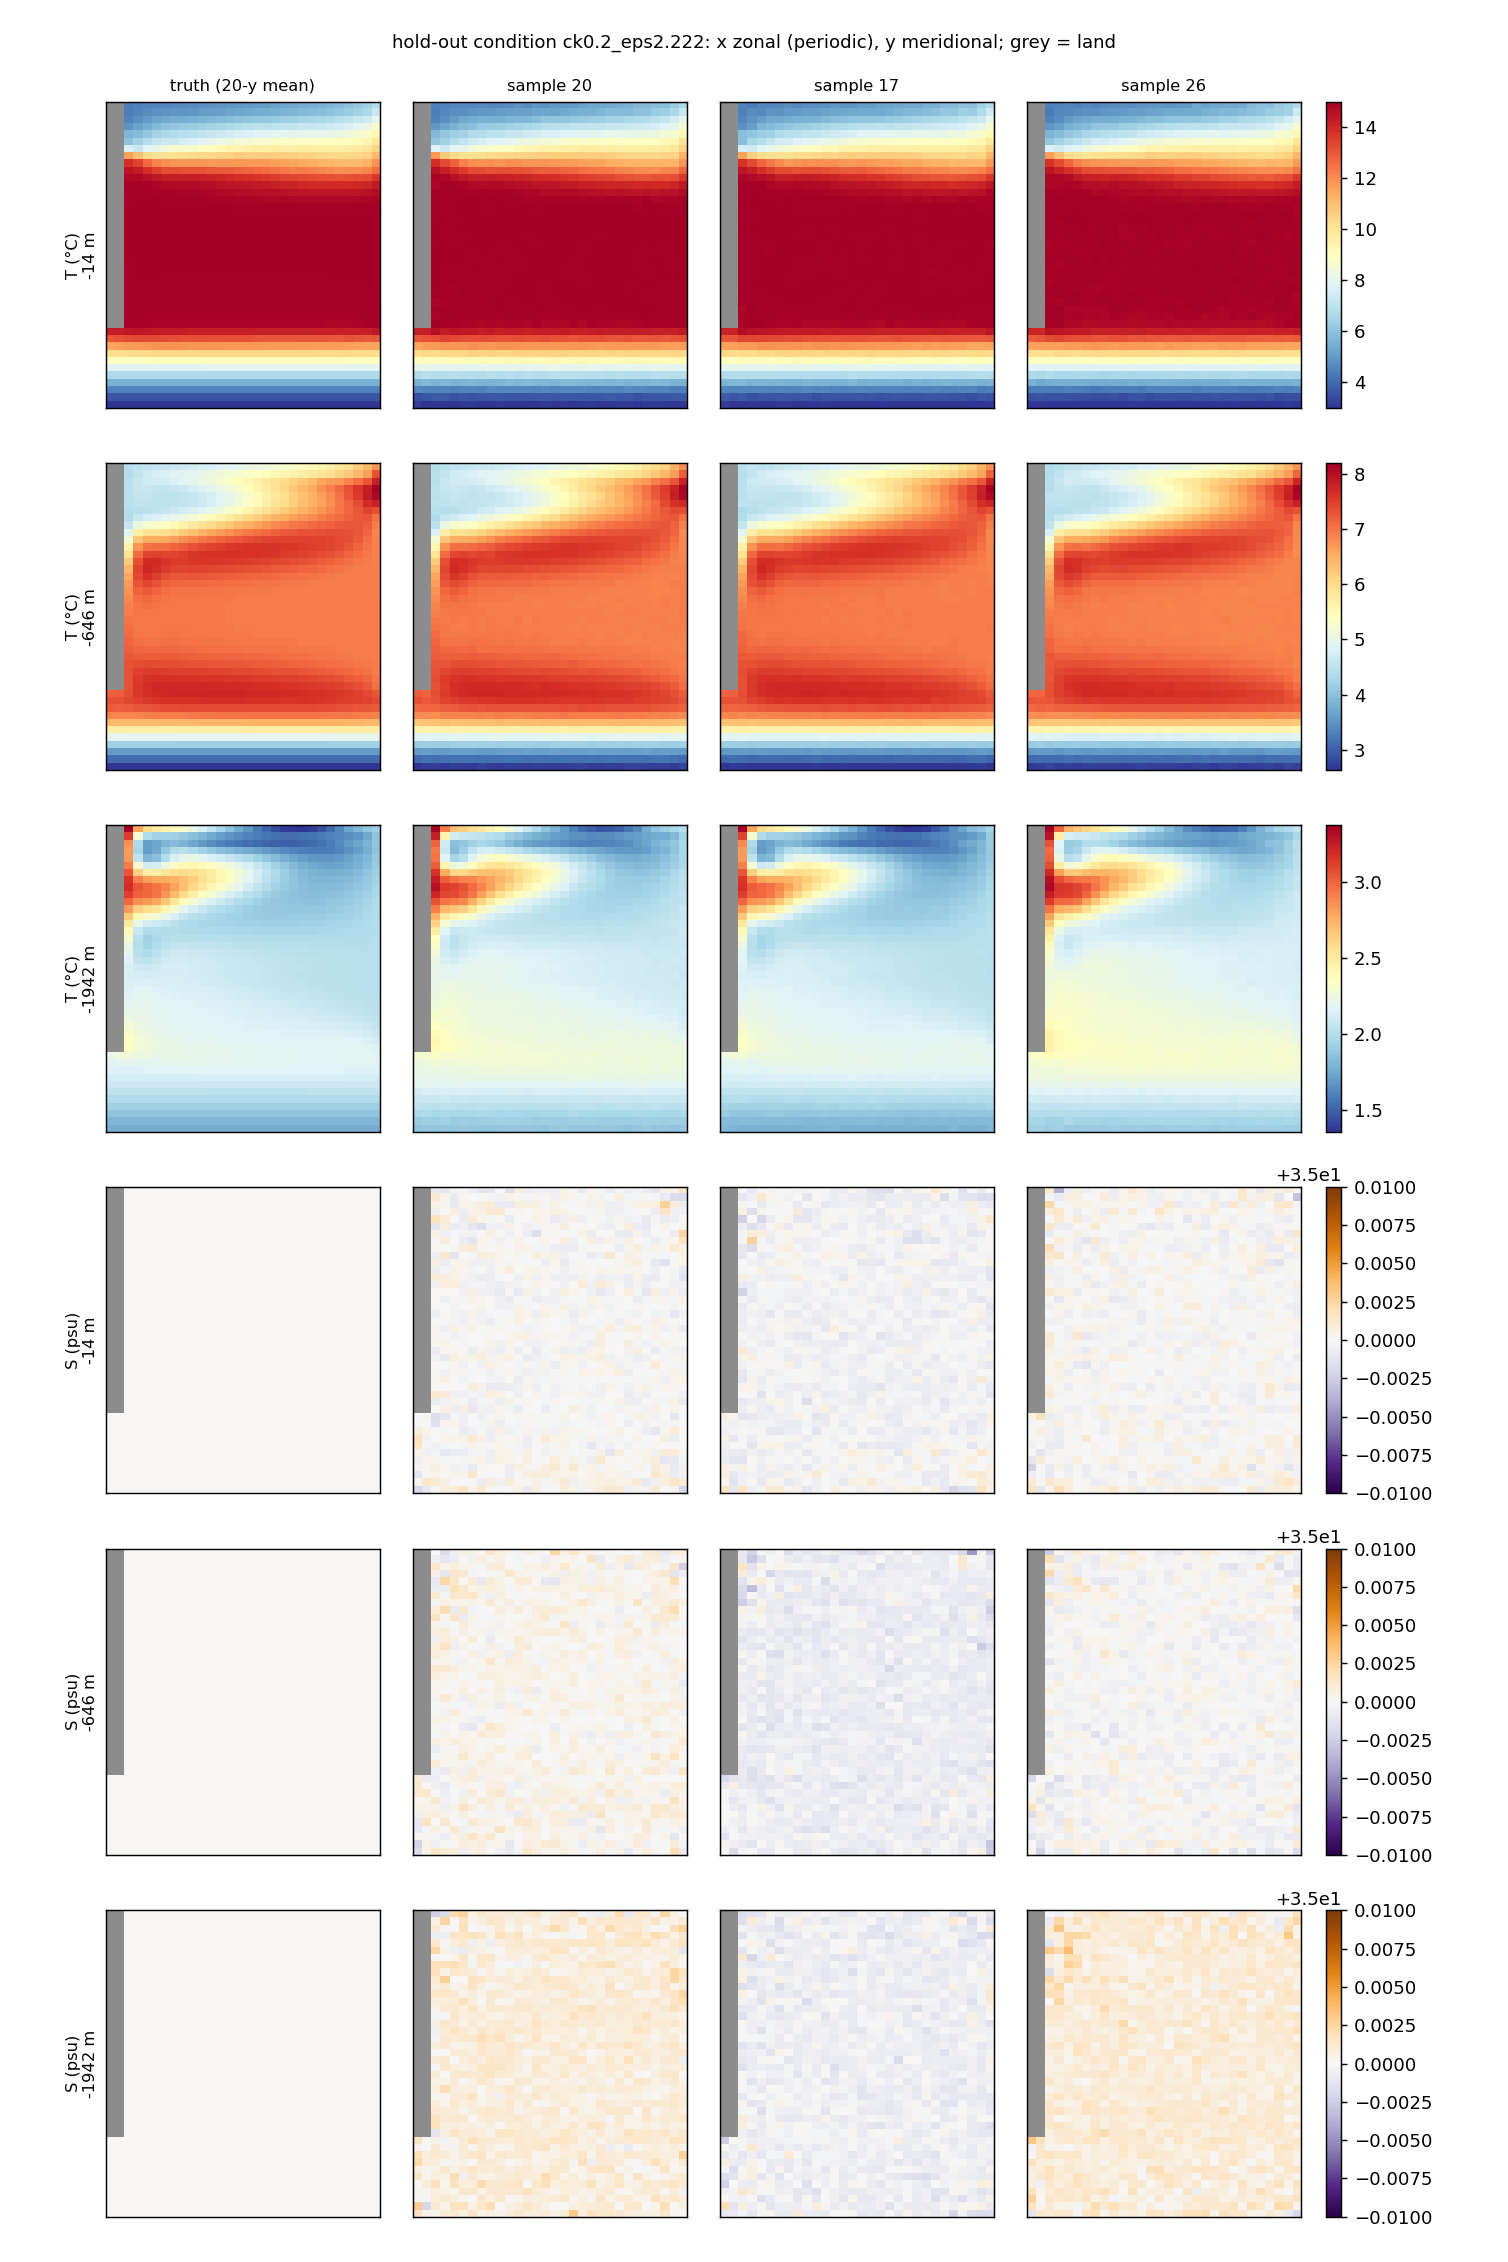
\includegraphics[width=0.9\textwidth]{../fs_block5_vml_3std/samples_levels.png}
\caption{True 20-year mean state and three random samples of $T$ and $S$ at the surface, \SI{646}{m} and the bottom for one held-out condition of the centre $5\times5$ split (grey: land; $x$ zonal and periodic, $y$ meridional).}
\label{fig:samples_block5}
\end{figure}

\begin{figure}[!htb]
\centering
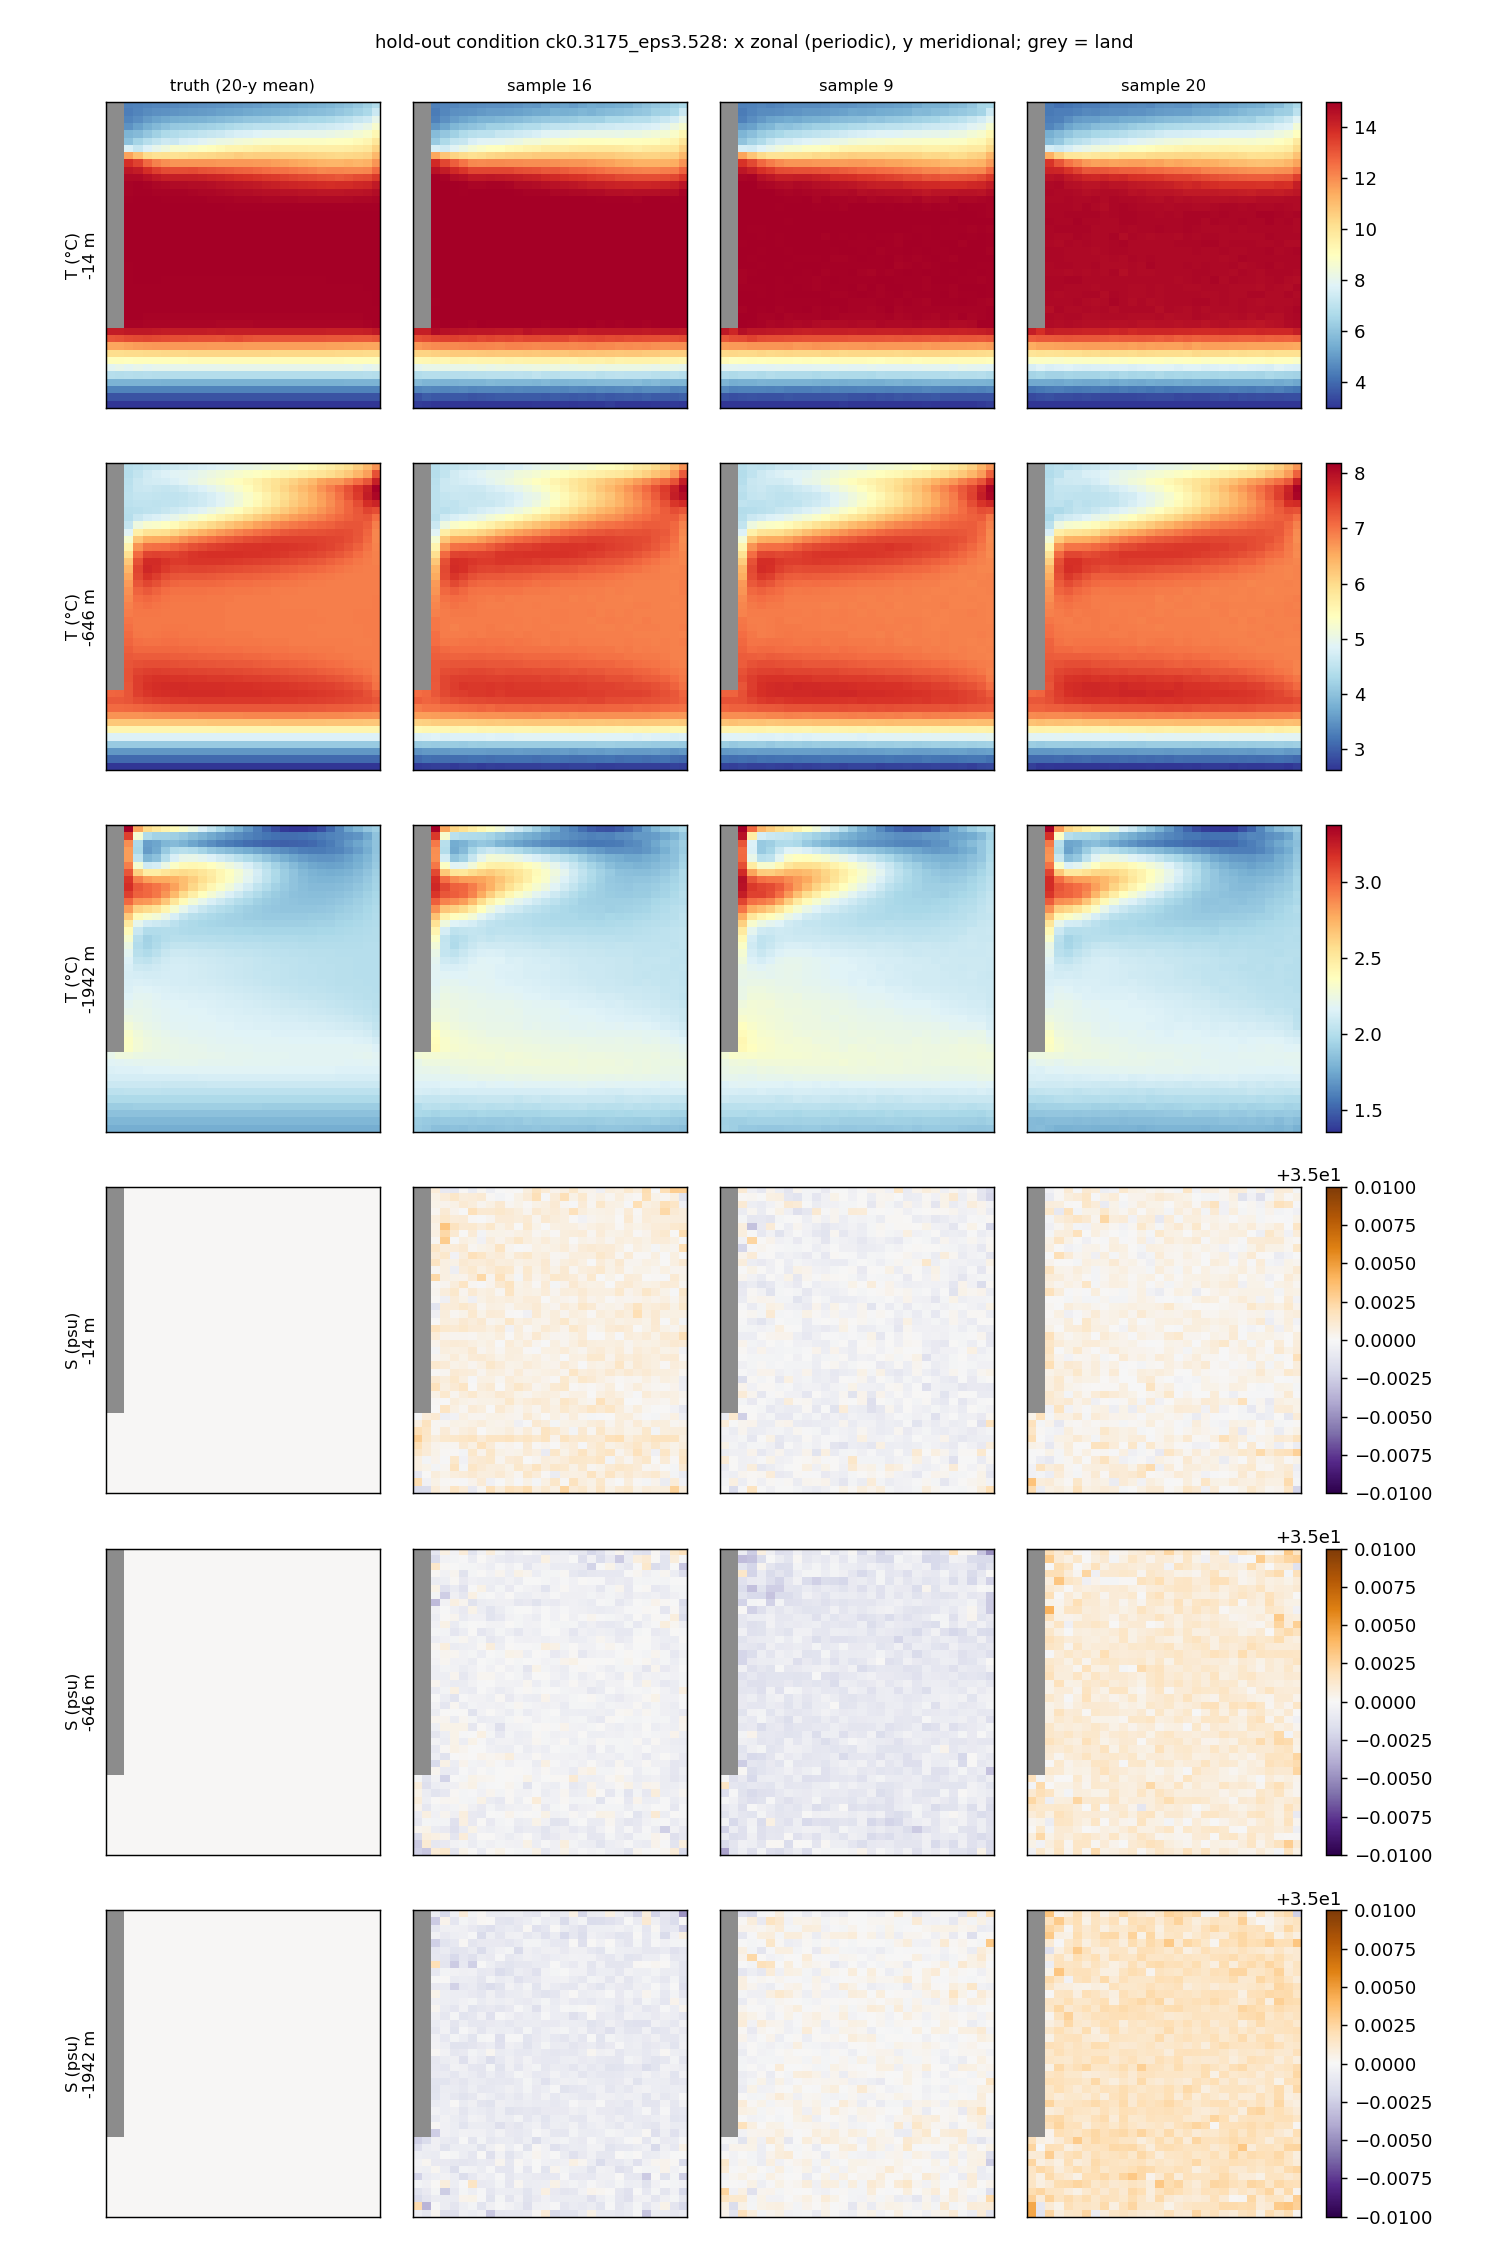
\includegraphics[width=0.9\textwidth]{../fs_block_vml_3std/samples_levels.png}
\caption{True 20-year mean state and three random samples of $T$ and $S$ at the surface, \SI{646}{m} and the bottom for one held-out condition of the centre $7\times7$ split (grey: land; $x$ zonal and periodic, $y$ meridional).}
\label{fig:samples_block}
\end{figure}

\begin{figure}[!htb]
\centering
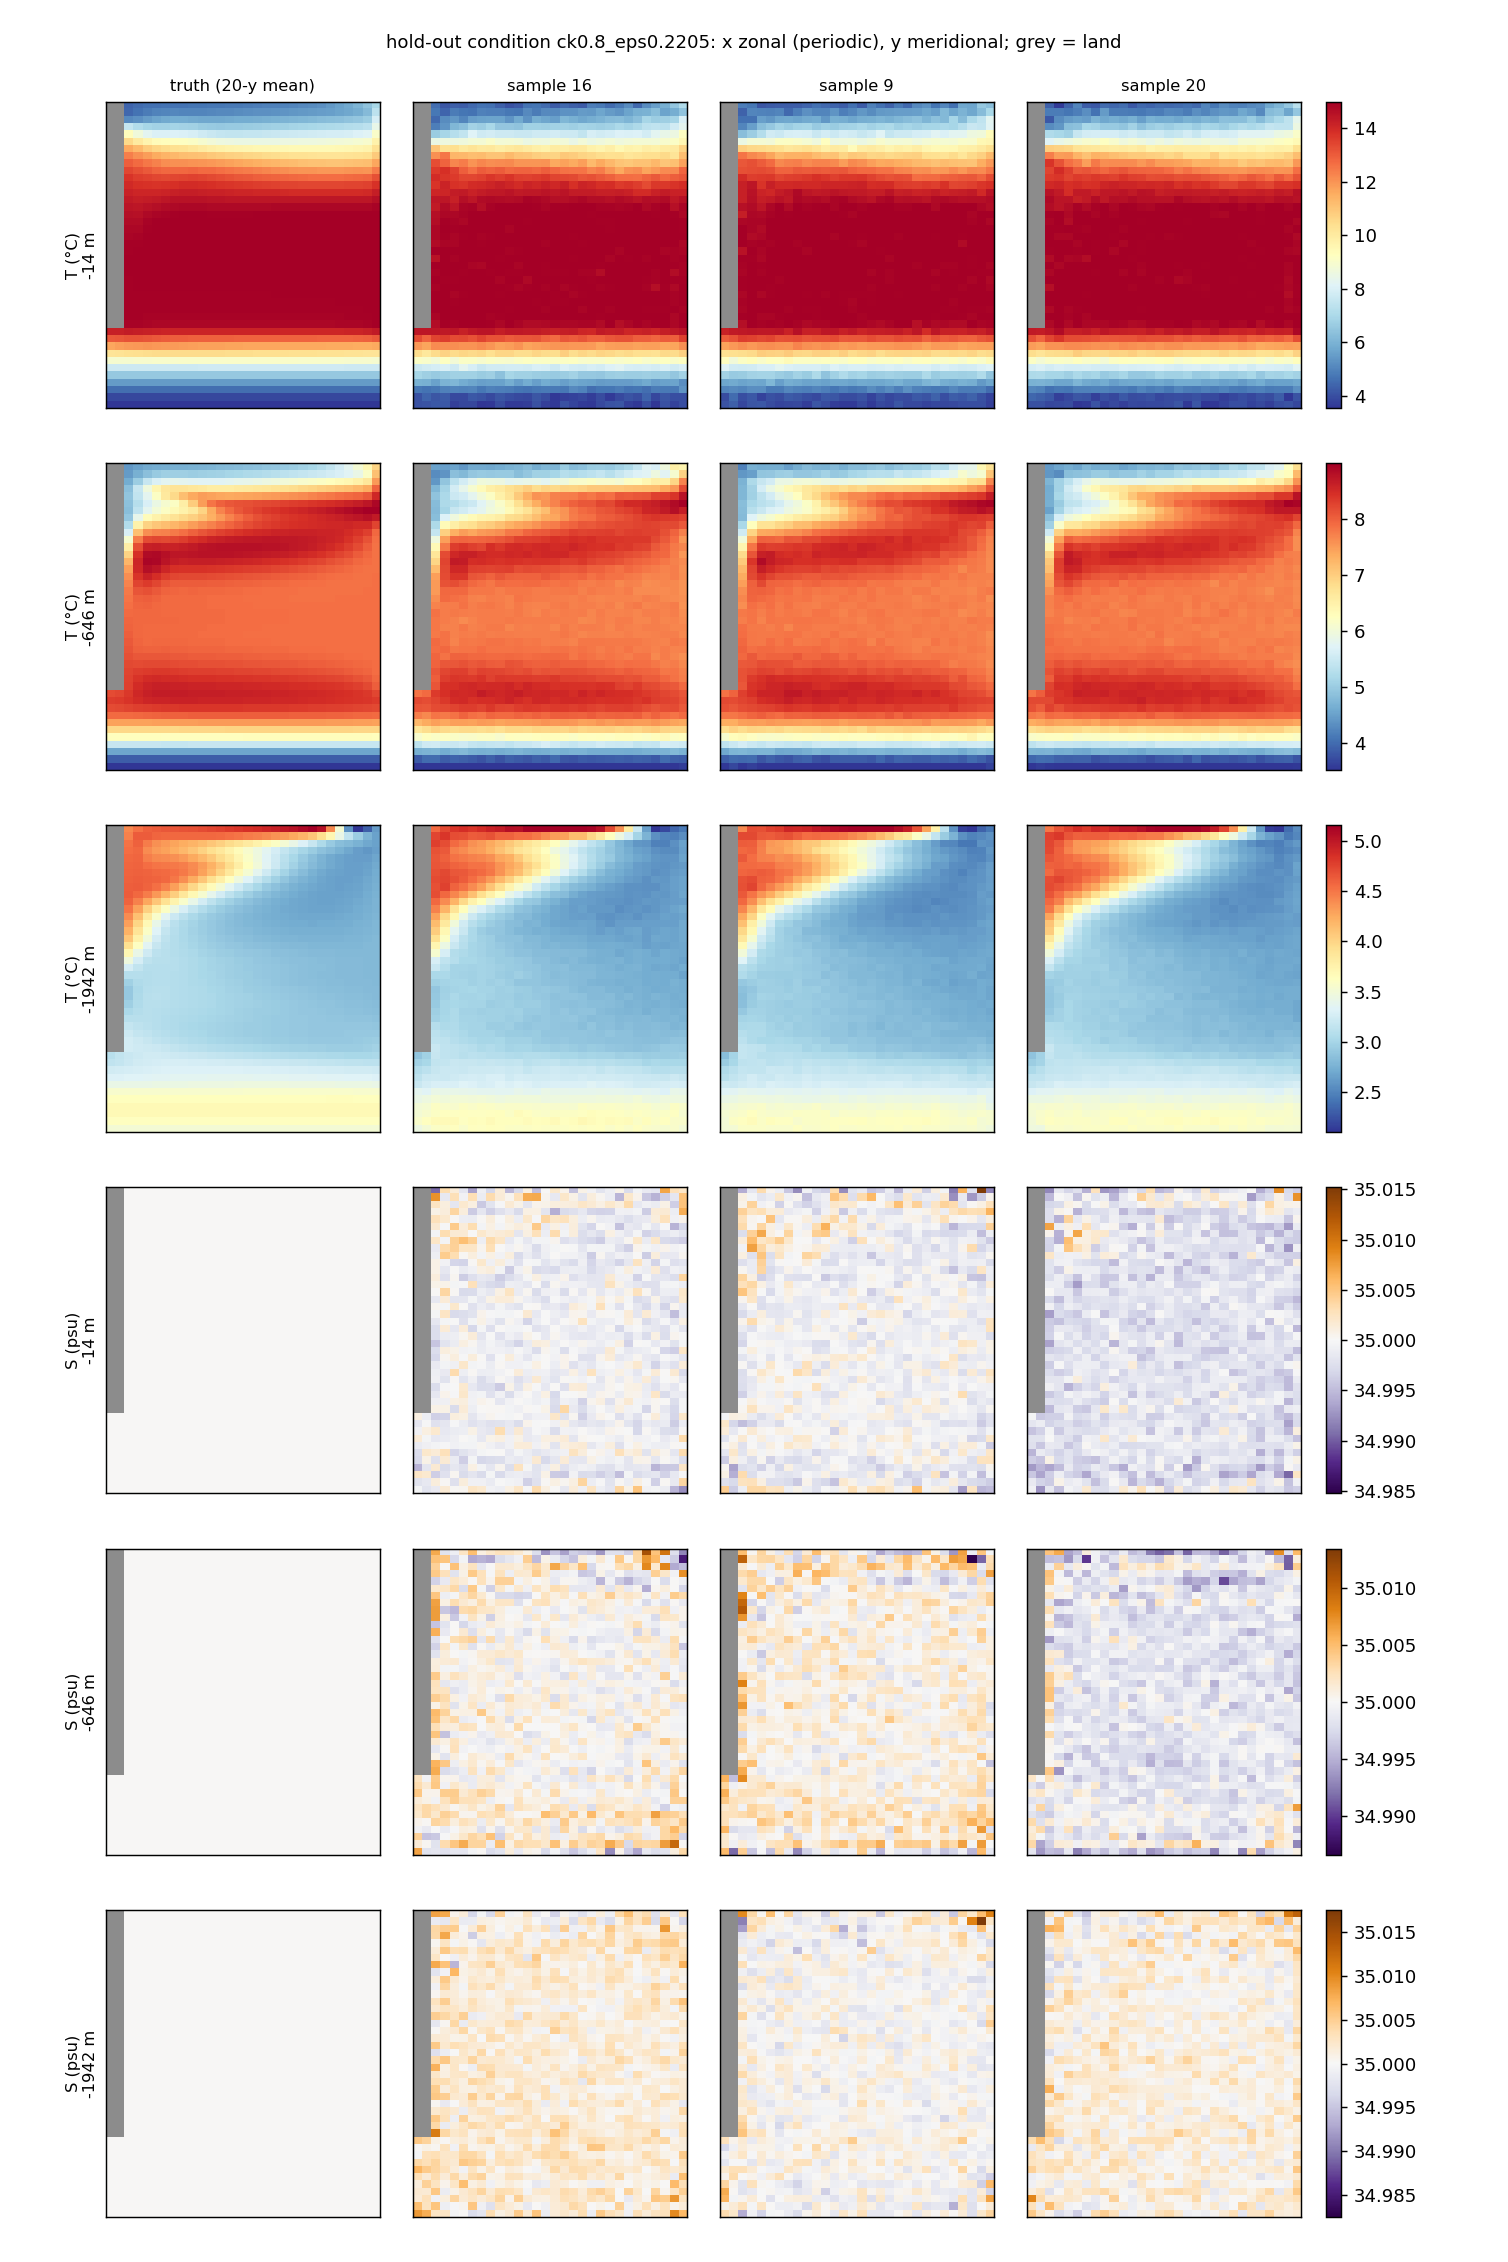
\includegraphics[width=0.9\textwidth]{../fs_ring_vml_3std/samples_levels.png}
\caption{True 20-year mean state and three random samples of $T$ and $S$ at the surface, \SI{646}{m} and the bottom for one held-out condition of the outer-51 split (grey: land; $x$ zonal and periodic, $y$ meridional).}
\label{fig:samples_ring}
\end{figure}

\begin{figure}[!htb]
\centering
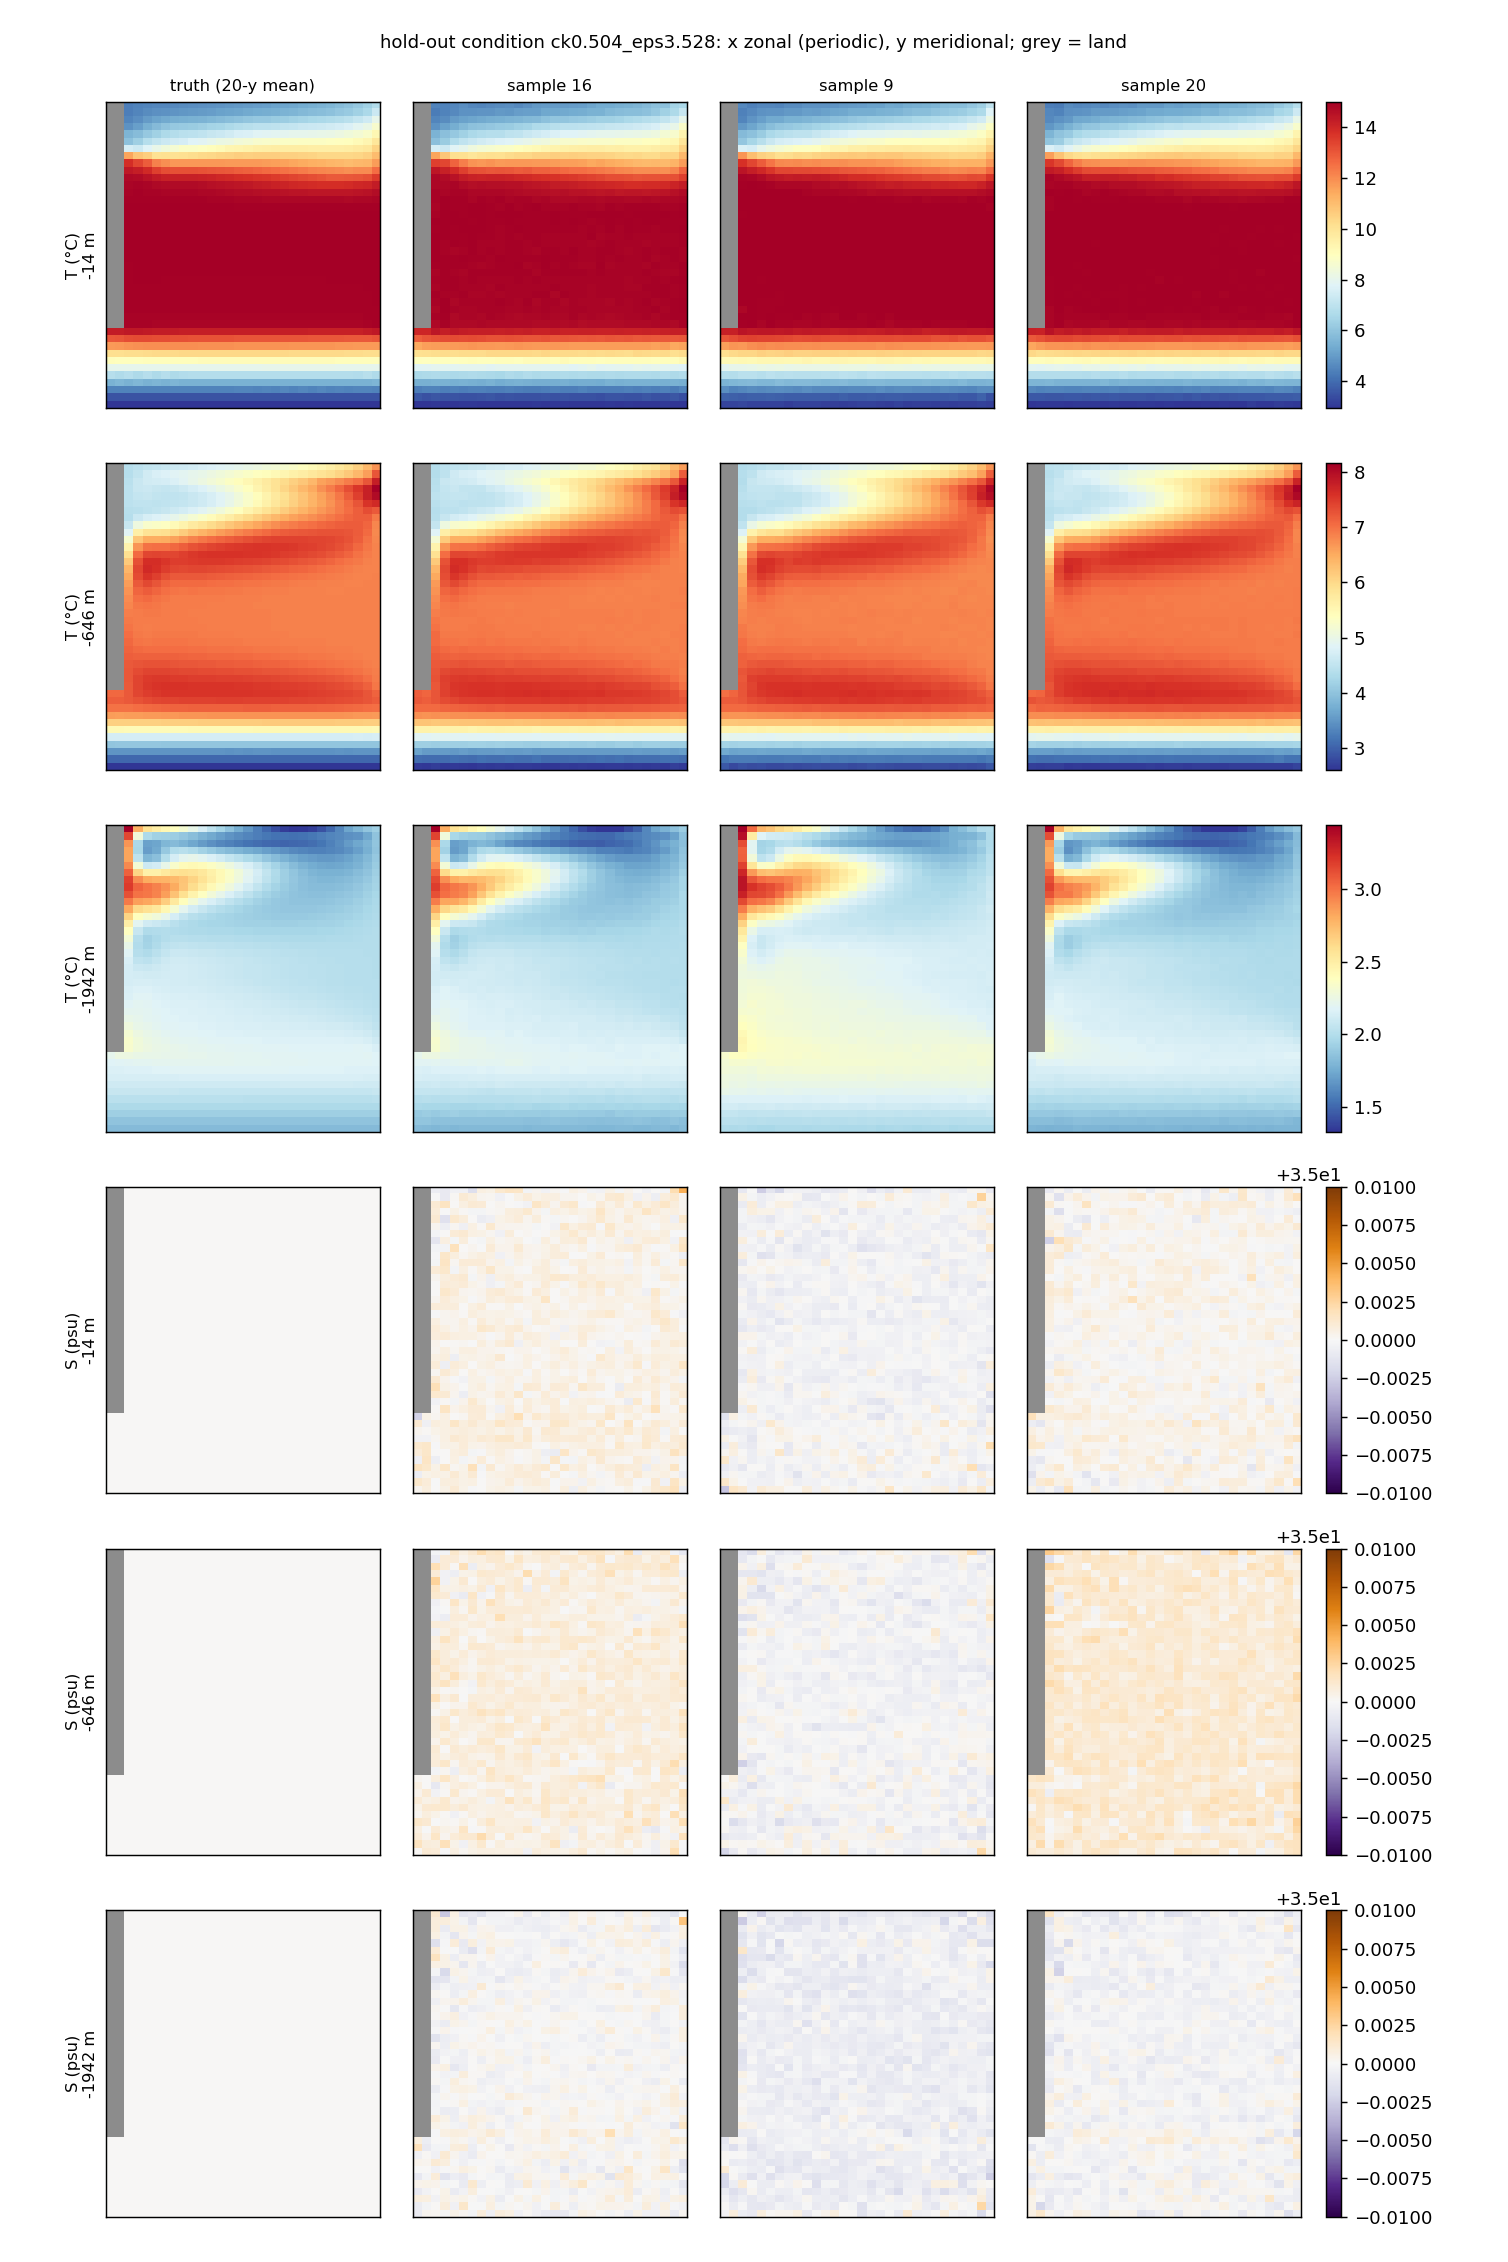
\includegraphics[width=0.9\textwidth]{../fs_ring5_vml_3std/samples_levels.png}
\caption{True 20-year mean state and three random samples of $T$ and $S$ at the surface, \SI{646}{m} and the bottom for one held-out condition of the outer-75 split (grey: land; $x$ zonal and periodic, $y$ meridional).}
\label{fig:samples_ring5}
\end{figure}

\begin{figure}[!htb]
\centering
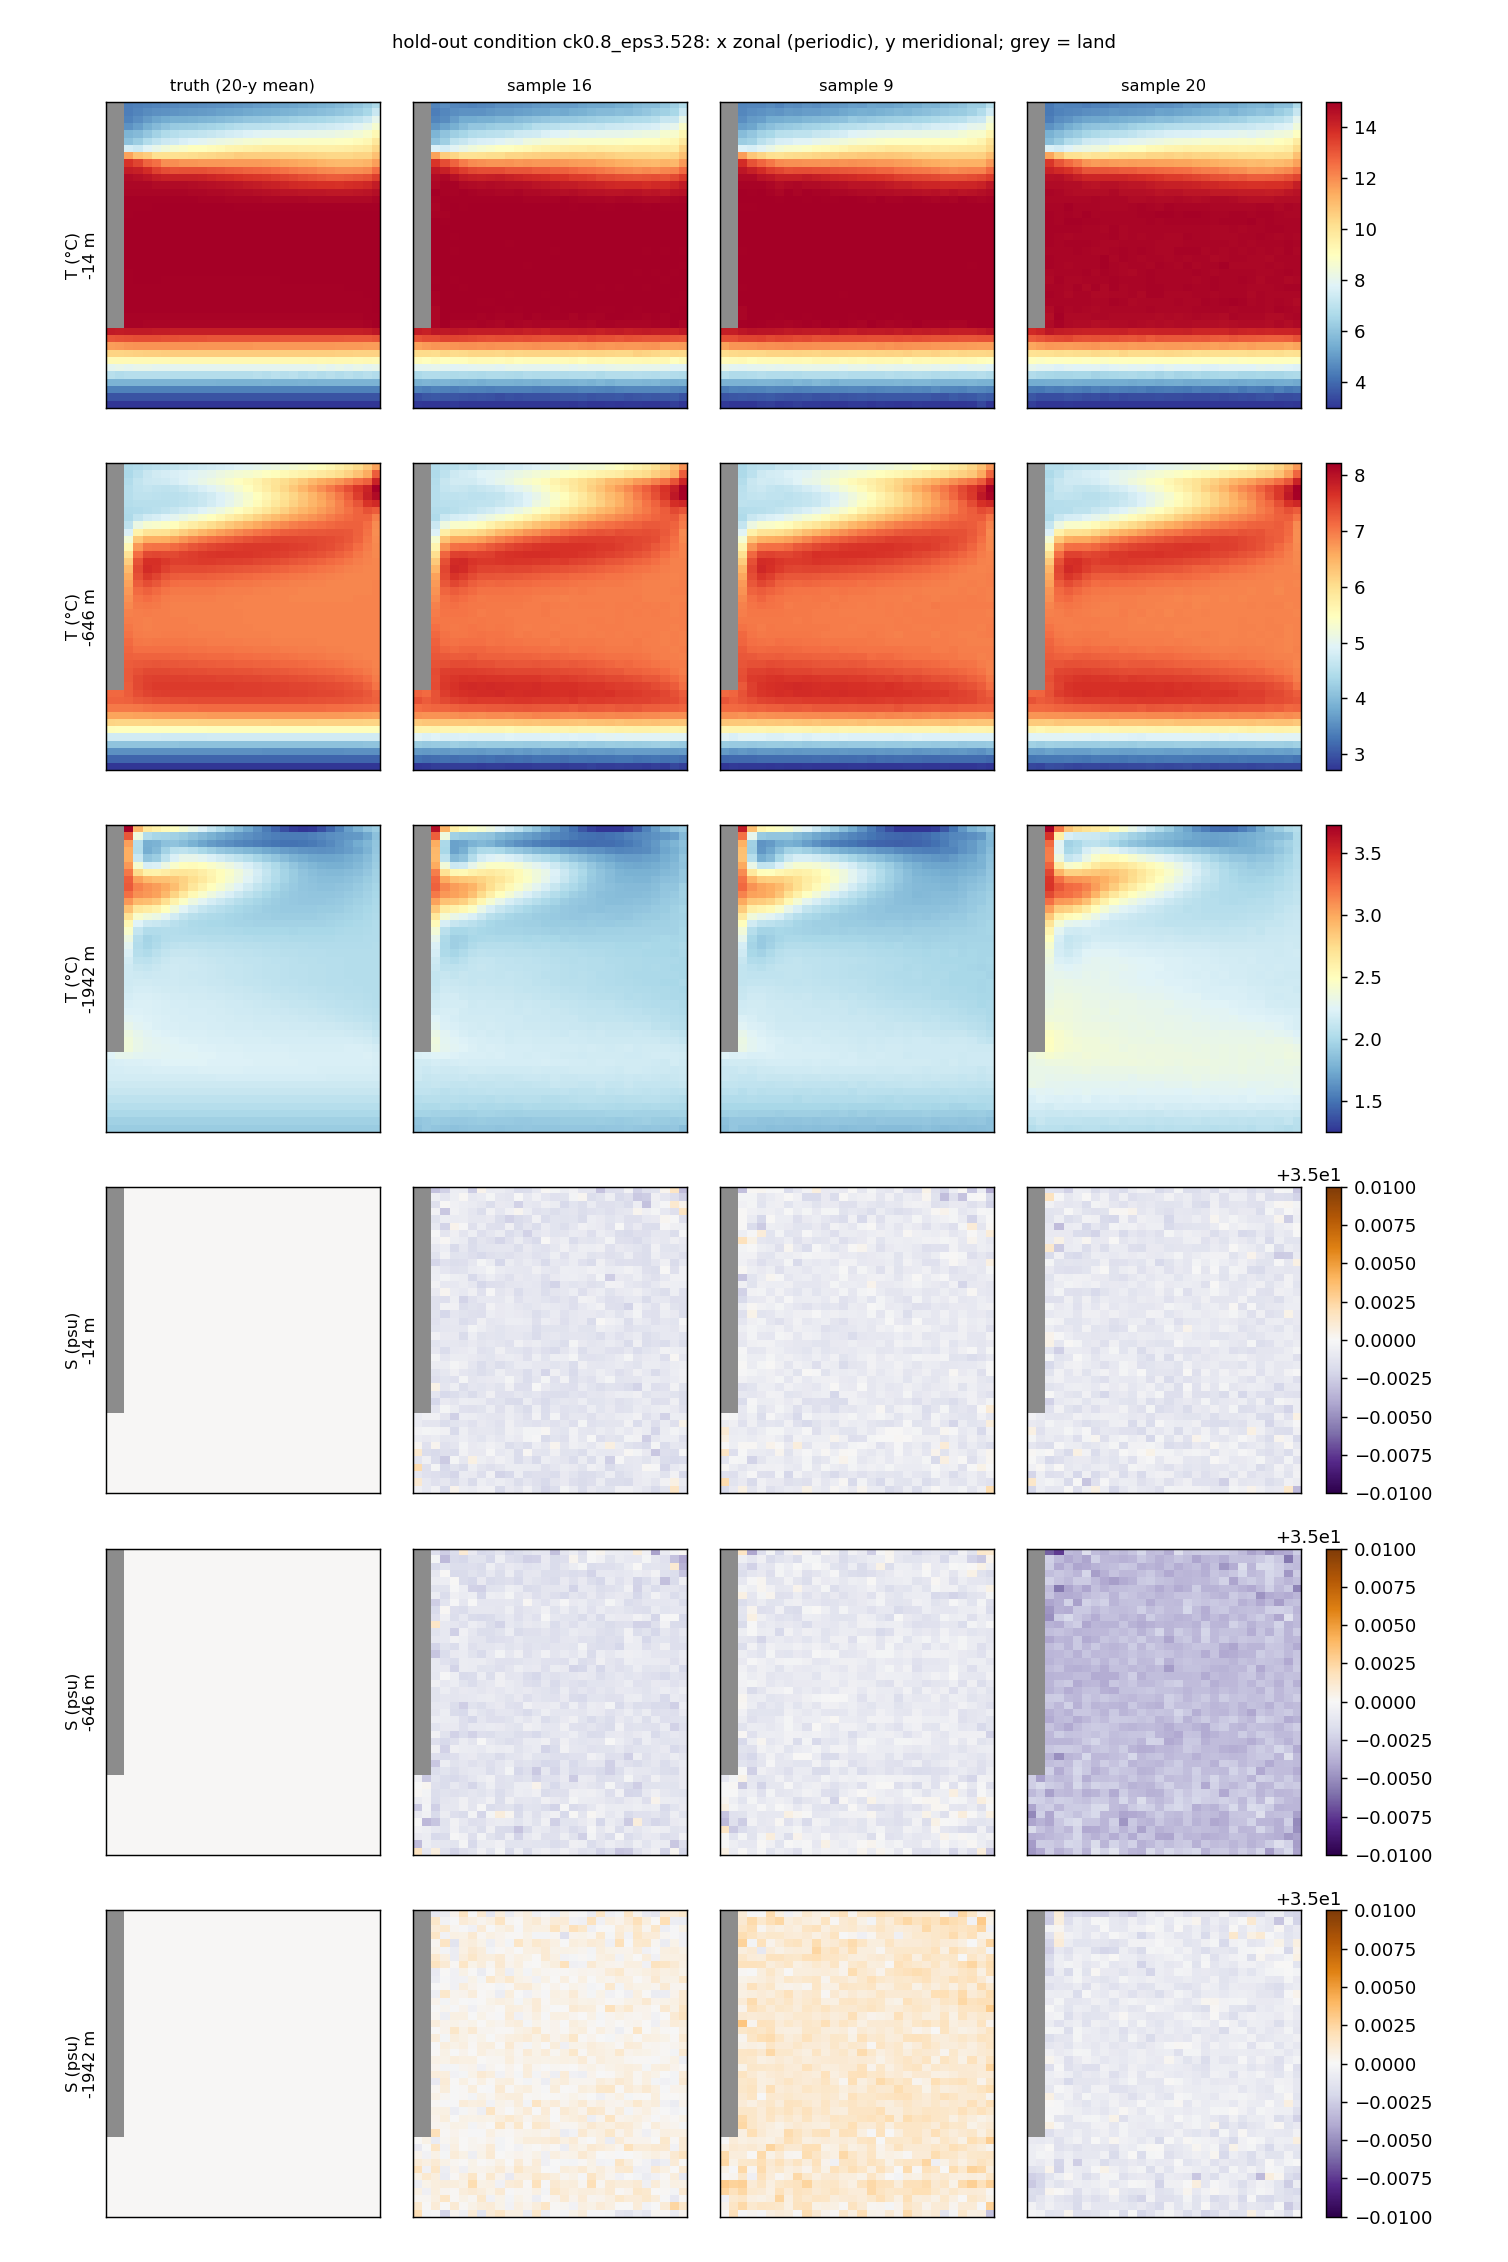
\includegraphics[width=0.9\textwidth]{../fs_top_vml_3std/samples_levels.png}
\caption{True 20-year mean state and three random samples of $T$ and $S$ at the surface, \SI{646}{m} and the bottom for one held-out condition of the top-row split (grey: land; $x$ zonal and periodic, $y$ meridional).}
\label{fig:samples_top}
\end{figure}

\begin{figure}[!htb]
\centering
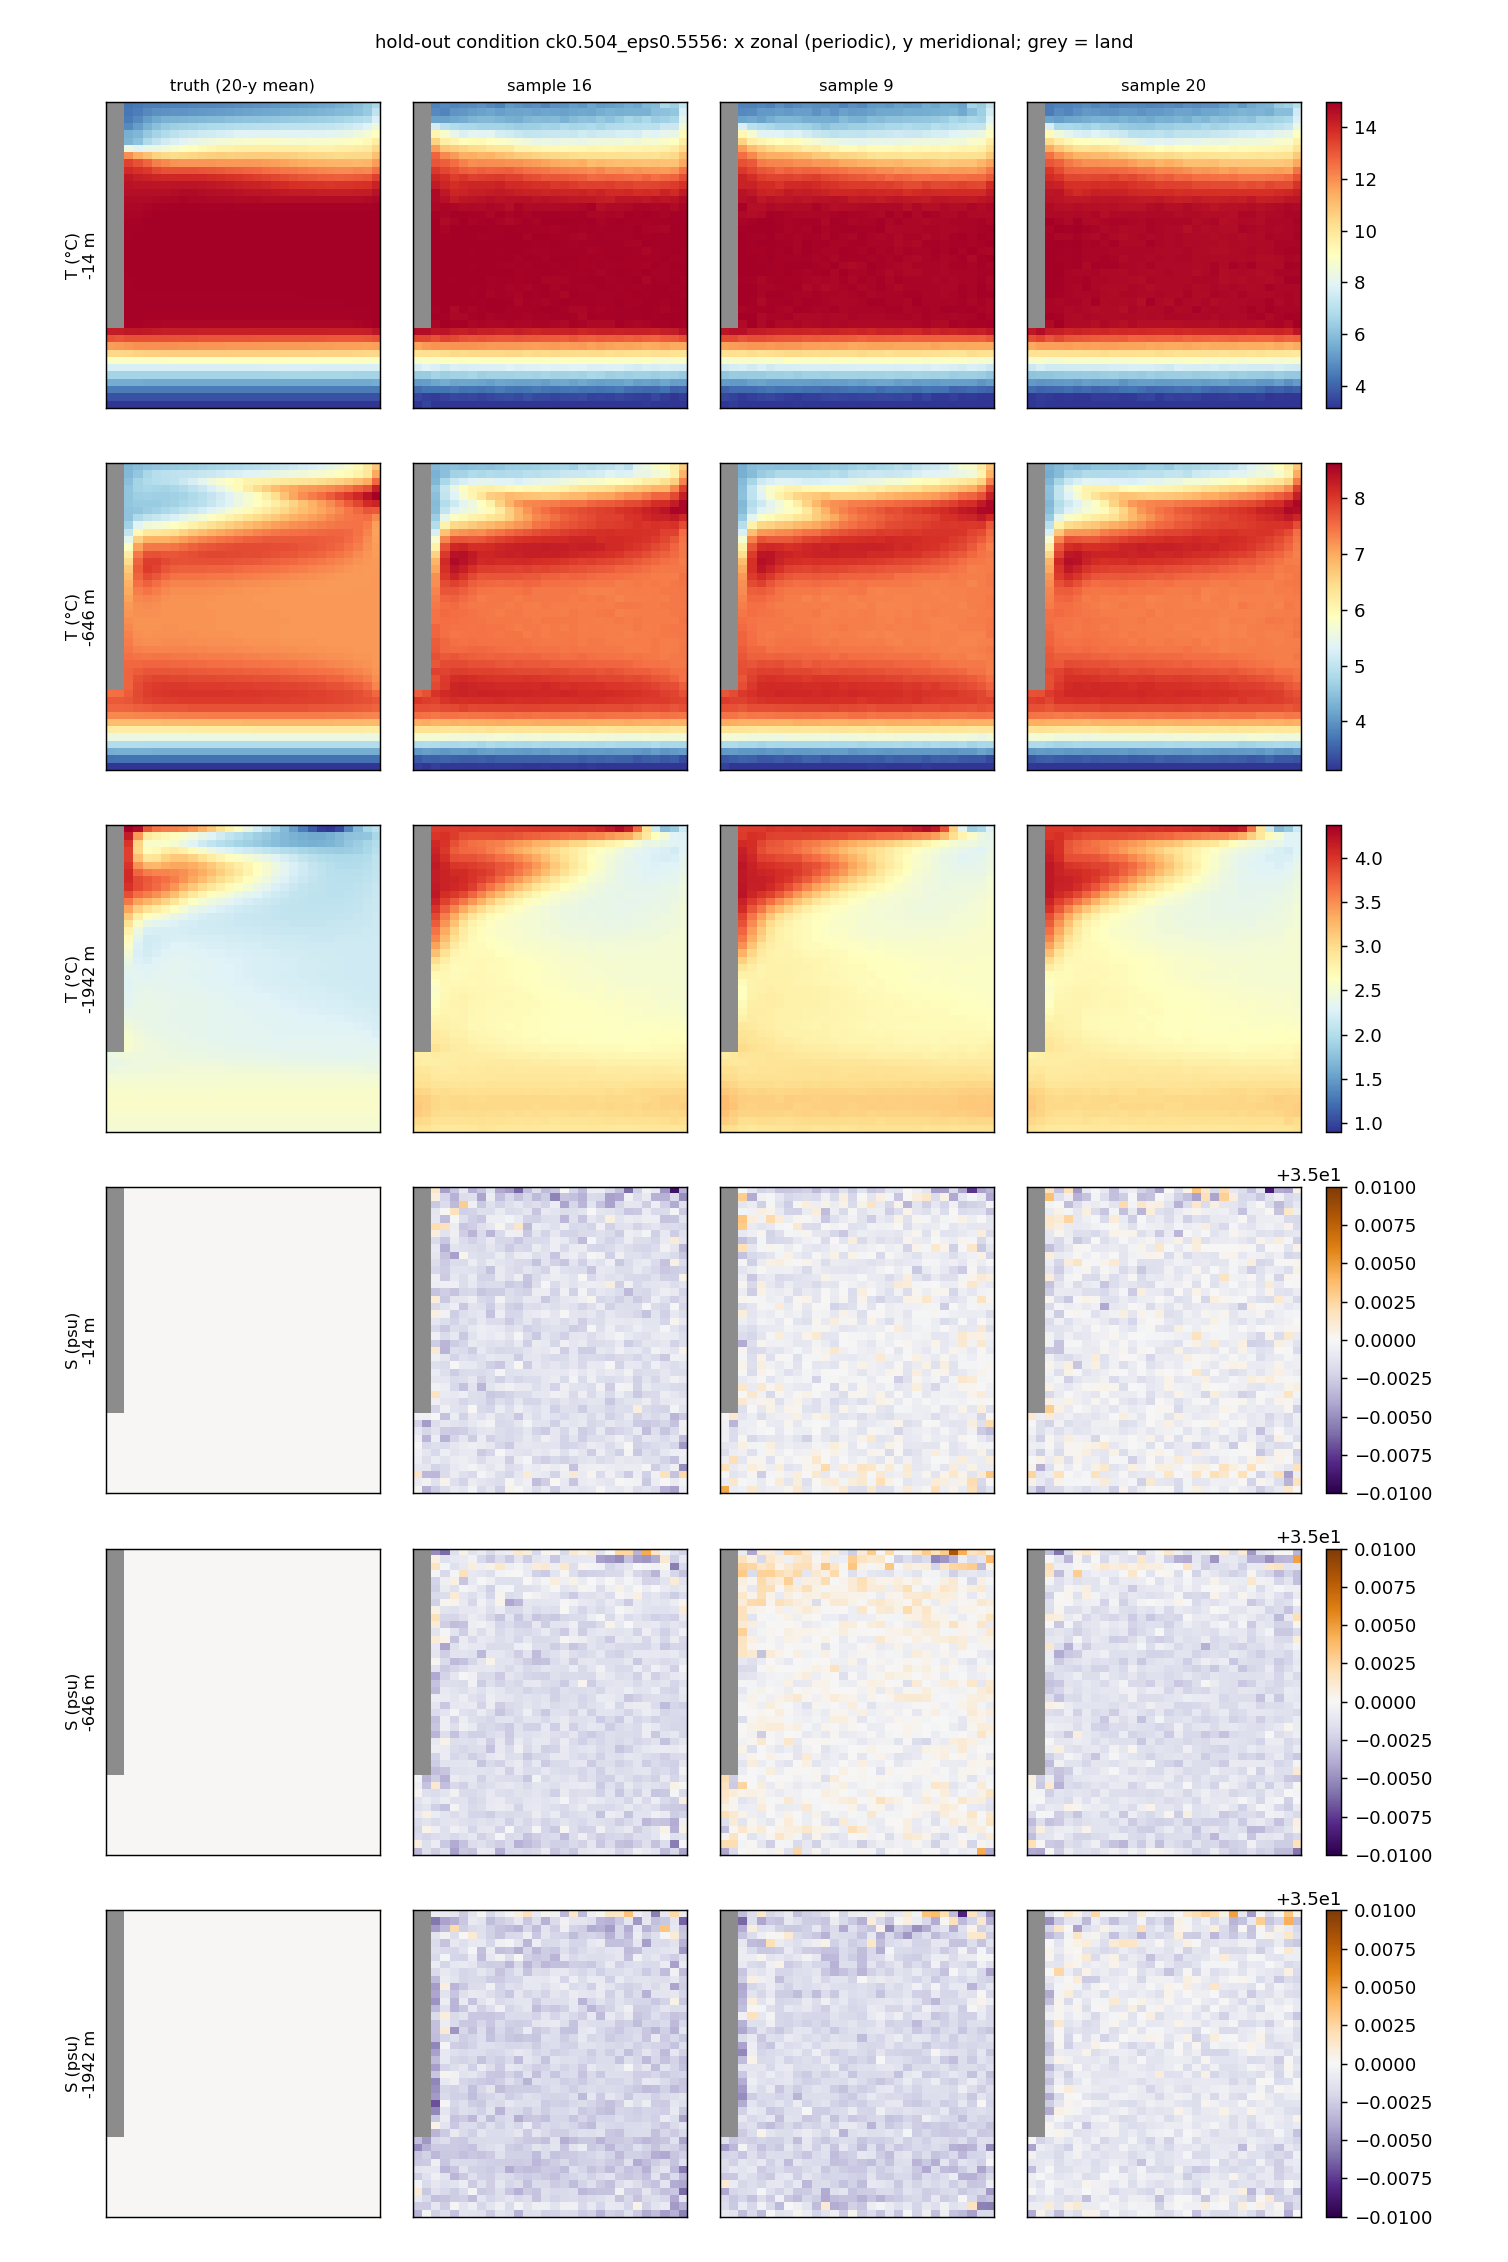
\includegraphics[width=0.9\textwidth]{../fs_four_vml_3std/samples_levels.png}
\caption{True 20-year mean state and three random samples of $T$ and $S$ at the surface, \SI{646}{m} and the bottom for one held-out condition of the four-run split (grey: land; $x$ zonal and periodic, $y$ meridional).}
\label{fig:samples_four}
\end{figure}

\begin{figure}[!htb]
\centering
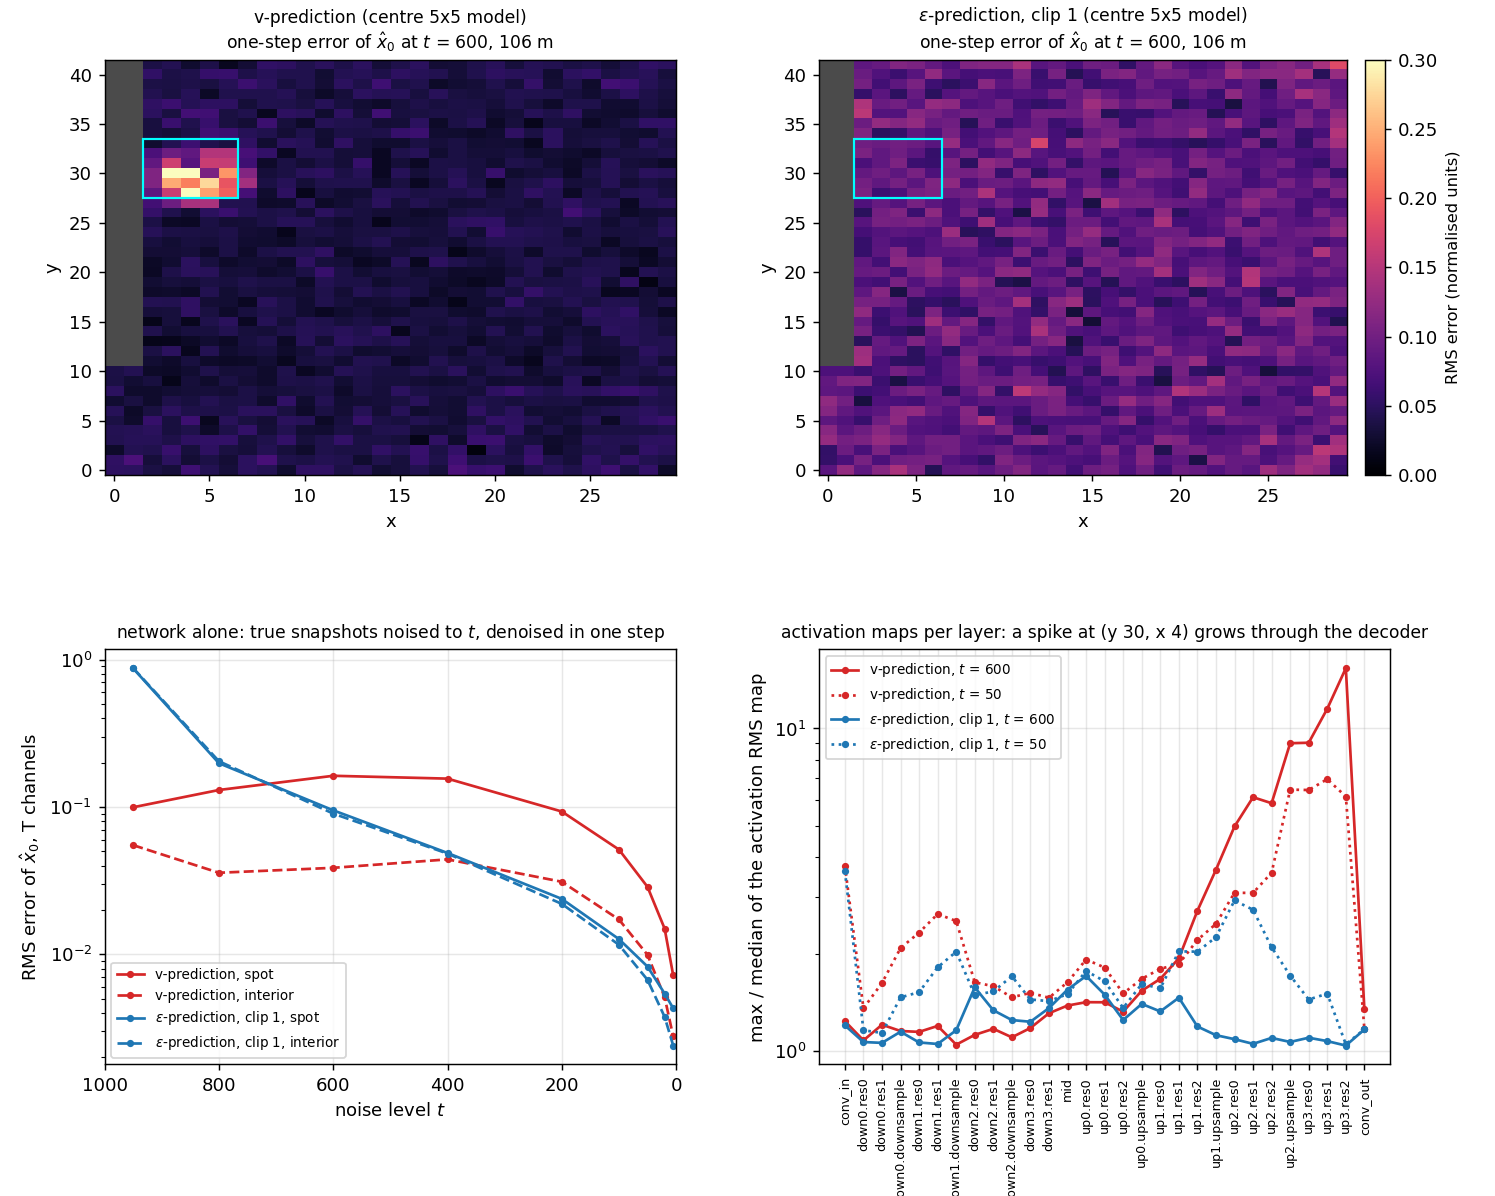
\includegraphics[width=\textwidth]{../fs_block5_v_3std/spot_diag.png}
\caption{The decoder spike of a velocity-target model trained with the loss on all cells (centre $5\times5$ split).
Top: RMS error of the one-step clean-state estimate for eight true snapshots of a held-out run noised to
$t$ = 600, at \SI{106}{m}, for that network (left) and for an $\epsilon$-prediction network (right); cyan box: the
patch. Bottom left: the same error in the patch and in an interior box as a function of $t$. Bottom right: maximum
over median of each layer's activation map: the spike appears in the second decoder block and grows through the
decoder. With the loss on the water cells the maps are flat and the patch is gone.}
\label{fig:spot}
\end{figure}

\end{document}
